% backup|Calculus A, B
\documentclass[12pt]{article}
% packages
\usepackage[paper=letterpaper,margin=1.6cm,bottom=0.8in]{geometry}
\usepackage[skip=5pt plus1pt, indent=15pt]{parskip}
\usepackage{amsmath}
\usepackage{amssymb}
\usepackage{amsfonts}
\usepackage{graphics}
\usepackage{graphicx}
\usepackage{newtxtext, newtxmath}
\usepackage{titling}
\usepackage{setspace}
\usepackage{titleps}
\usepackage[x11names]{xcolor}
\colorlet{shadecolor}{LavenderBlush3}
\usepackage{annotate-equations}
\usepackage{framed}

\usepackage[colorlinks=true, linkcolor=violet]{hyperref}

% settings
\newpagestyle{mypage}{%
% make head rule gray
    \headrule
  \sethead{\textcolor{gray}{\thesubsection}}{}{\textcolor{gray}{\sectiontitle: \subsectiontitle}}
  \setfoot{}{\textcolor{gray}{\thepage}}{}
}

\setlength{\droptitle}{-6em}
\onehalfspacing


\begin{document}
% commands
\newcommand{\red}[1]{\textcolor{red}{#1}}
\newcommand{\ddx}{\frac{d}{dx}}
\newcommand{\ddy}{\frac{d}{dy}}
\newcommand{\dxdy}{\frac{dx}{dy}}
\newcommand{\dydx}{\frac{dy}{dx}}
\newcommand{\pd}[2]{\frac{\partial #1}{\partial #2}}

\newcommand{\real}{\mathbb{R}}
\newcommand{\naturals}{\mathbb{N}}
\newcommand{\integers}{\mathbb{Z}}
\newcommand{\rational}{\mathbb{Q}}
\newcommand{\complex}{\mathbb{C}}

\begin{titlepage}
    \begin{center}
        \vspace*{1cm}
        \Huge
        \textbf{Calculus I, II, III}
        
        \vfill
        
        \begin{figure}[!ht]
            \centering
            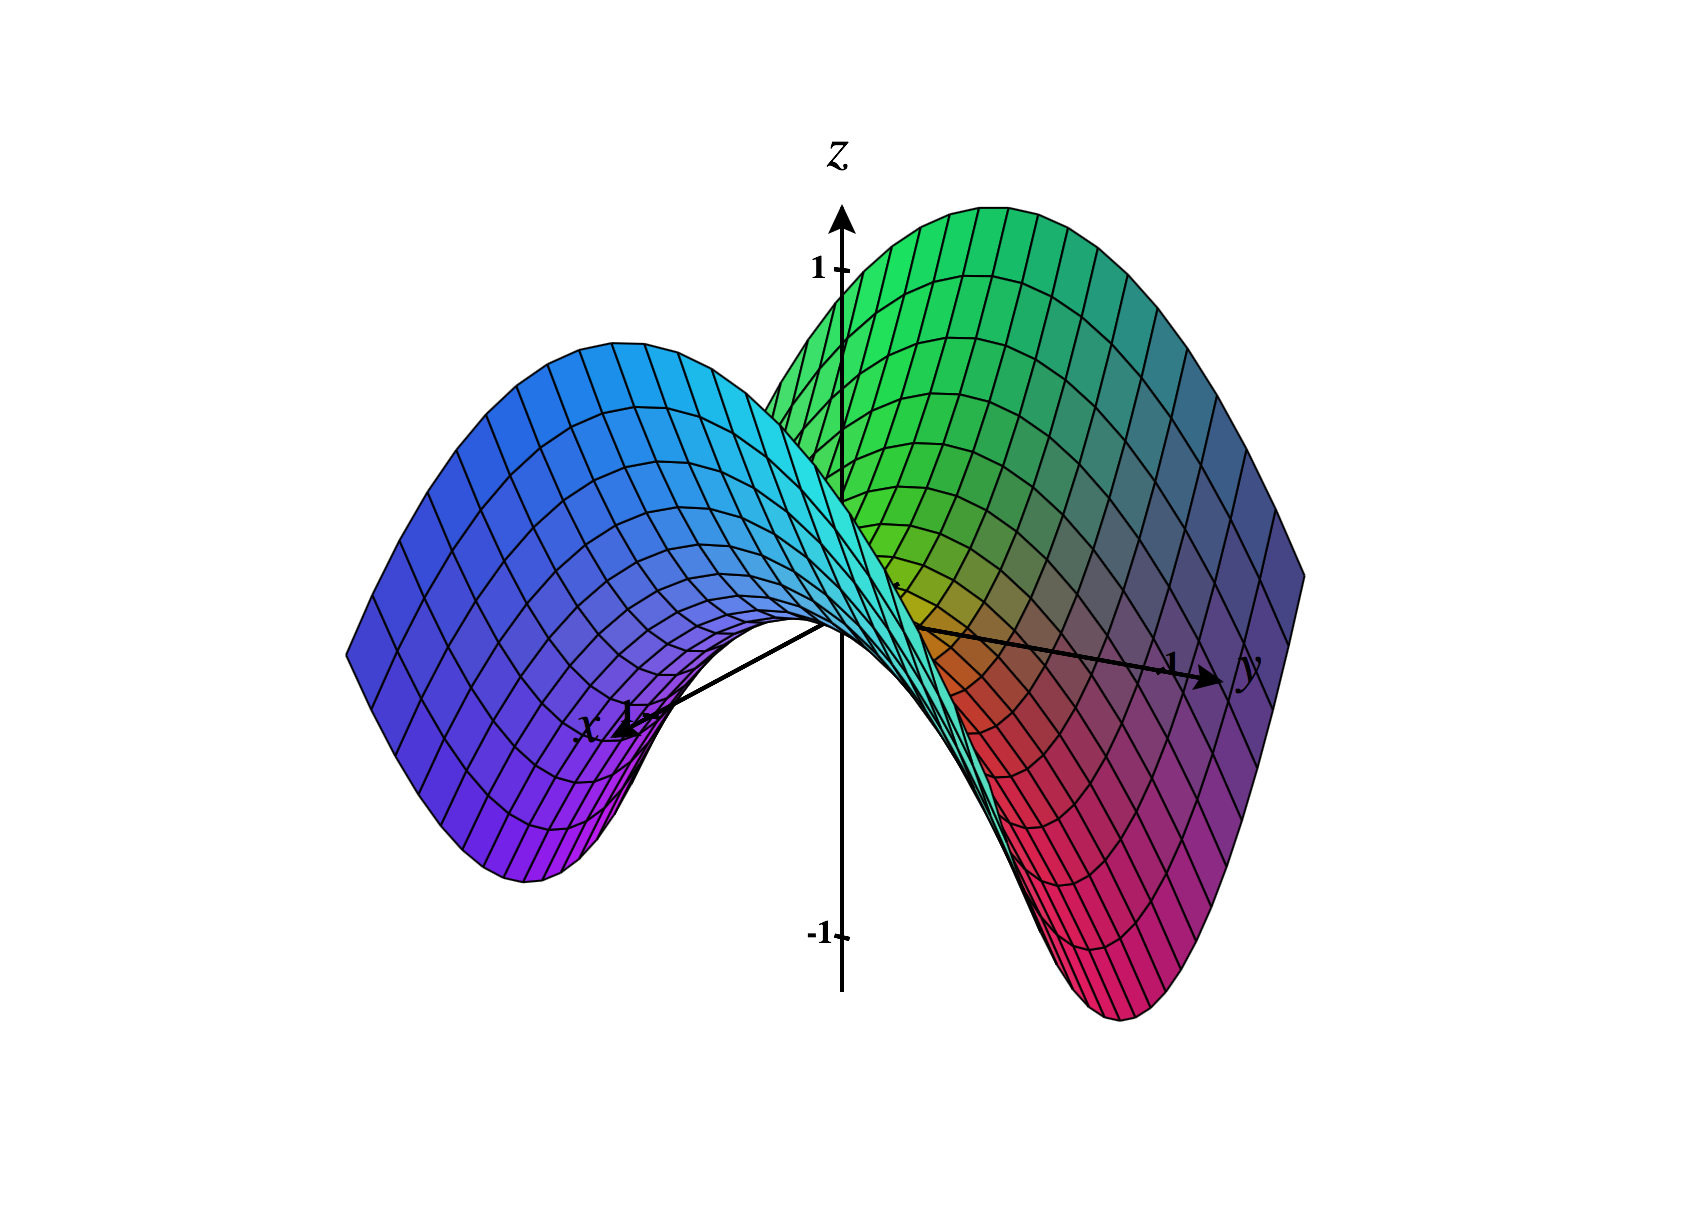
\includegraphics[width=17cm]{misc/saddle.png}
        \end{figure}
        \vfill
        
        \small
        by Louis Meunier
        
        \href{https://notes.louismeunier.net}{\color{violet}{notes.louismeunier.net}}
        
    \end{center}
\end{titlepage}

{
  \hypersetup{linkcolor=violet}
  \tableofcontents
}

\newpage
\pagestyle{mypage}
\section{Limits}
\subsection{Tricks for solving limits}
\setlength\itemsep{5em}
\subsubsection{\texorpdfstring{$\frac{x}{x}$}{TEXT}}

In some situations, you can multiply a limit by some factor of $\frac{x}{x}$ to simplify an otherwise "impossible" limit

eg:
\begin{equation}
\begin{split}
    \lim_{x\to\infty} \frac{x+3}{\sqrt{9x^2-5x}}
     & = \lim_{x\to\infty} \frac{x+3}{\sqrt{9x^2-5x}} . \textcolor{red}{\frac{\frac{1}{x}}{\frac{1}{x}}}\\
     & = \lim_{x\to\infty} \frac{\frac{x}{x}+\frac{3}{x}}{\sqrt{(\frac{1}{x^2})(9x^2-5x)}}\\
     & = \lim_{x\to\infty} \frac{1+\frac{3}{x}}{\sqrt{9-\frac{5}{x}}}
 \end{split}
\end{equation}      
The terms $\frac{3}{x}$ and $\frac{5}{x}$ both tend to $0$ as $x \to \infty$, so the final limit simplifies:
\begin{equation}
\begin{split}
    \lim_{x\to\infty} \frac{1}{\sqrt{9}}
     & = \frac{1}{\sqrt{9}}\\
     & = \frac{1}{3}
 \end{split}
\end{equation}  

\subsubsection{Intuition with \texorpdfstring{$\infty$}{TEXT}}

In limits involving fractions where both numerator and denominator are polynomials, you can intuitively calculate the limit using the coefficients/powers.

$$
    \lim_{x\to\infty} \frac{ax^{m}}{bx^n}
$$
\begin{enumerate}
    \item $\mathbf{m > n}:$ $\infty$
    \item $\mathbf{m < n}:$ $0$ 
    \item $\mathbf{m = n}:$  $\frac{m}{n}$ \textit{(since both of the powers are the same "strength" ie $\infty$, you can think of this as the infinities "canceling out"). To prove this idea actually works, use the method above.}
\end{enumerate}

\subsubsection{L'Hôpital's Rule}

\begin{shaded}
In short, if:
$$\frac{f(c)}{g(c)} = \frac{0}{0}, \frac{\infty}{\infty}, 0^0, \infty - \infty, ... (\textbf{indeterminate form})$$ 

then:
$$\lim_{x\to c}\frac{f(x)}{g(x)} = \lim_{x\to c}\frac{f'(x)}{g'(x)}$$
\end{shaded}
This can also be repeated for multiple derivatives of $f, g$, as long as the resulting form is still indeterminate. Oftentimes, you will need to manipulate the limit to express it in an indeterminate form such that L'Hôpital's is usable.

\textit{While solving limits this way is very powerful (and, often, very easy), one should be careful to not overuse it when it is not applicable.}

\subsubsection{Solving for a given limit}

When given a function with variables in place of constants and a final limit to solve for, there are some additional considerations to take into account.

eg:

$$\lim_{x\to0}\frac{\sqrt{ax + b} - 2}{x} = 1$$

In order for this limit to even exist, $\lim_{x\to0} \sqrt{ax + b} - 2$ MUST equal 0, following the quotient rule of limits, which states:

$$\lim_{x\to c} \frac{f(x)}{g(x)} = \frac{\lim_{x\to c} f(x)}{\lim_{x\to c} g(x)}$$

So:
\begin{equation}
\begin{split}
    \lim_{x\to0} \sqrt{ax + b} - 2 = 0\\
    \sqrt{a*0 + b} - 2 = 0\\
    \sqrt(b) = 2\\
    b = 4
\end{split}
\end{equation}
To finish solving this limit, see:

\subsubsection{"Radicalizing" fraction}

Similar to the first point, but a little more complex/situation-specific.

When a limit is in the form:

$$\lim_{x\to 0}\frac{\sqrt[n]{(ax+b)} + c}{x}$$

The issue here is that we have an $x$ alone on the bottom, which results in something being divided by 0. To solve this, we can radicalize the fraction; this results in an $x$ "alone", canceling with that on the bottom, making the equation solvable.

For the example above:
\begin{equation}
\begin{split}
    \lim_{x\to0} \frac{\sqrt{ax + 4} - 2}{x} = 1\\
    \lim_{x\to0} \frac{\sqrt{ax + 4} - 2}{x}.\textcolor{red}{\frac{\sqrt{ax + 4} + 2}{\sqrt{ax + 4} + 2}} = 1\\
    \lim_{x\to0} \frac{a\textcolor{red}{x}}{\textcolor{red}{x}(\sqrt{ax+4}+2)} = 1\\
    \lim_{x\to 0} \frac{a}{\sqrt{ax + 4} + 2} = 1\\
    ...\\
    a = 4
\end{split}
\end{equation}
\subsubsection{Squeeze Theorem}

\begin{shaded*}
If: 
    \begin{itemize}
        \item $f(x) \leq g(x) \leq h(x)$ 

        \item $\lim_{x \to c} f(x) = \lim_{x \to c} h(x)$

    \end{itemize}
then $\lim_{x\to c} f(x) = \lim_{x \to c} g(x) = \lim_{x \to c} h(x)$
    
\end{shaded*}

This makes a lot more sense in practice:

\begin{equation}
    \begin{split}
        \lim_{x\to0} x^4 sin(\frac{x}{2}) = ?\\
        -1 \leq sin(\frac{x}{2}) \leq 1\\
        -x^4 \leq x^4 sin(\frac{x}{2}) \leq x^4\\
        \lim_{x\to 0} -x^4 = \lim_{x\to 0} x^4 = 0 \therefore \lim_{x\to0} x^4 sin(\frac{x}{2}) = 0
    \end{split}
\end{equation}

See Figure \ref{squeeze} to see this visually.

\begin{figure}[!ht]
    \centering
    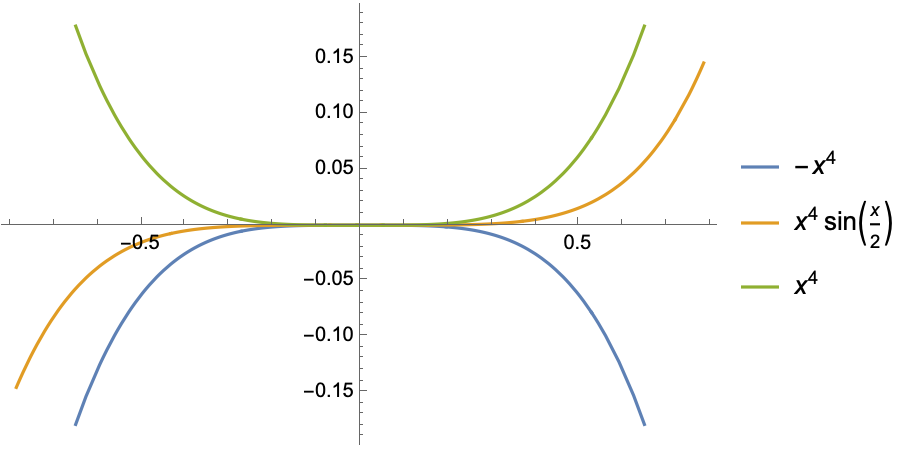
\includegraphics[width=12.0cm]{misc/squeezetheorem.png}
    \caption{The squeeze theorem visualized}
    \label{squeeze}
\end{figure}

\subsubsection{Using the definition of a derivative}

A derivative, $f'(x)$, is defined as followed:

$$f'(x) = \lim_{x\to a}\frac{f(x)-f(a)}{x-a}$$

Alternatively, given $h = x-a$:

$$f'(x) = \lim_{h\to 0} \frac{f(x+h)-f(h)}{h}$$

If you are given a limit in the form (or near) the above forms, you can use these definitions to solve the limit. 

eg: 

\begin{equation}
    \begin{split}
    \lim_{x\to \pi}\frac{e^{sin(x)} - 1}{x - \pi} &= \lim_{x\to \pi}\frac{e^{sin(x)} - \textcolor{red}{e^{sin(\pi)}}}{x - \pi}\\
    \textit{Let f(x) = $e^{sin(x)}$}\\
    &=\lim_{x\to \pi}\frac{f(x)-f(\pi)}{x - \pi}\\
    \textit{This is simply the definition of $f'(x)$ at $a=\pi$}\\
    &=f'(\pi) = cos(\pi)e^{sin(\pi)} = -1
    \end{split}
\end{equation}

\subsection{Intermediate Value Theorem}
\begin{shaded}
    If
    \begin{itemize}
        \item $f$ is continuous on $[a,b]$
        \item $f(a) \neq f(b)$
        \item $f(a) <= N <= f(b)$
    \end{itemize}

    there exists some $c$ in $(a,b)$ such that $N = f(c)$.
    
    See Figure \ref{ivt}.
\end{shaded}
\begin{figure}[!ht]
    \centering
    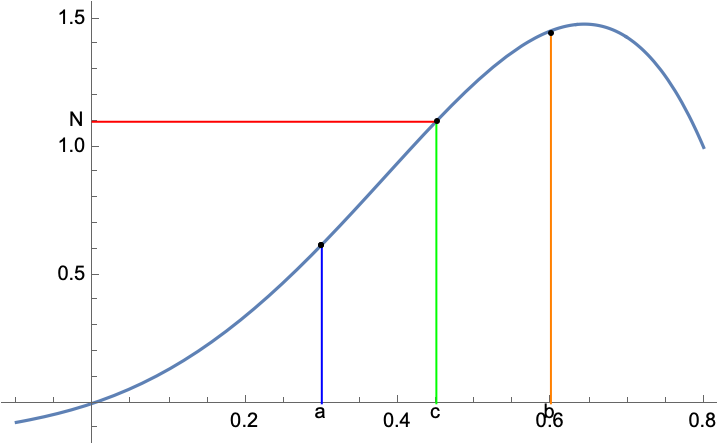
\includegraphics[width=10.0cm]{misc/imvt.png}
    \caption{The intermediate value theorem visualized}
    \label{ivt}
\end{figure}

\section{Exponential and Logarithmic Functions}
\subsection{Exponential Functions}
\subsubsection{Defining \texorpdfstring{$e$}{TEXT}}

An exponential function is any $f(x)$ of the form $f(x) = a^x$. To find the derivative, $f'(x)$:

\begin{equation}
    \begin{split}
        f'(x) &= \lim_{h\to 0} [\frac{a^{x+h}-a^x}{h}]\\
        &=\textcolor{red}{a^x}\lim_{h\to 0}[\frac{a^h-1}{h}]\\
    \end{split}
\end{equation}

We can rewrite this for the derivative of $f$ at $x = 0$:

\begin{equation}\label{eqn:expderiv}
    \begin{split}
    f'(0) &= \textcolor{red}{a^0}\lim_{h\to 0}[\frac{a^h-1}{h}]\\
    &=\lim_{h\to 0}[\frac{a^h-1}{h}]
    \end{split}
\end{equation}

We can use this to find for what value of $a$ that $f'(0) = f(0)$. $f(0) = a^0 = 1$, therefore $f'(0) = f(0) = 1 = \lim_{h\to 0}[\frac{a^h-1}{h}]$.

\begin{equation}
    \begin{split}
        1 &= \lim_{h\to 0}[\frac{a^h-1}{h}]\\
        \mathbf{a = 2:} \lim_{h\to 0}[\frac{2^h-1}{h}] &= 0.693...\\
        \mathbf{a = 3:} \lim_{h\to 0}[\frac{2^h-1}{h}] &= 1.099...\\
    \end{split}
\end{equation}

By the Intermediate Value Theorem, we know that $2 < a < 3$, which can be defined by $e$.

\begin{equation}\label{eqn:edef}
    \begin{split}
        1 = e^0 = \lim_{h\to 0}[\frac{\textcolor{red}{e}^h-1}{h}]
    \end{split}
\end{equation}
Extending this further for e;

\begin{equation}\label{exp:fullexpderiv}
    \begin{split}
        \frac{d}{dx} e^x &= \lim_{h\to 0}[\frac{e^{x+h}-e^x}{h}]\\
        &= e^x \textcolor{red}{\lim_{h\to 0}[\frac{e^h-1}{h}]}\\
        \textit{Substituting from eqn. \ref{eqn:edef}}\\
        &= \mathbf{e^x}
    \end{split}
\end{equation}

\subsubsection{Generalizing \texorpdfstring{$\frac{d}{dx} a^x$}{TEXT}}

From eqn. \ref{eqn:expderiv}:

$$\frac{d}{dx}a^x = a^x \lim_{h\to 0} \frac{a^h-1}{h} = f'(0) a^x$$

We can rewrite using the rules of logs:

$$\frac{d}{dx}a^x = \frac{d}{dx}\textcolor{red}{ e^{\ln a^x} } = \frac{d}{dx} e^{x\ln a}$$

We can let $u = x \ln a$, and thus $a^x = e^u$. We can then use implicit differentiation as follows:

\begin{equation}\label{exp:derivativeexpa}
    \begin{split}
        \frac{d}{dx} a^x &= \frac{d}{dx} e^u\\
        &=\frac{du}{dx} \frac{d}{du} [e^u]\\
        \textit{From eqn. \ref{exp:fullexpderiv}}\\
        &=e^u \frac{du}{dx}\\
        &= e^u \frac{d \textcolor{red}{(x \ln a)}}{dx}
        \textit{Differentiating in terms of x}\\
        &= e^u \ln a\\
        &= e^{\ln a^x} \ln a\\
        &= a^x \ln a\\
    \end{split}
\end{equation}

Thus, $\frac{d}{dx} a^x = a^x \ln a$.

\subsection{Logarithmic Functions}

Let $f(x) = y = \log_a{x}$, so $x = a^y$. To find the derivative of $f(x)$:

\begin{equation}
    \begin{split}
        \frac{d}{dx} x &= \frac{d}{dx} a^y\\
        1 &= [\frac{d}{dy} a^y] \frac{dy}{dx}\\
        \textit{Using eqn. \ref{exp:derivativeexpa}}:\\
        1 &= a^y \ln a \frac{dy}{dx}\\
        \frac{1}{a^y \ln a} &= \frac{dy}{dx}\\
        \textit{Subbing in for $y$}:\\
        \frac{1}{a^{\textcolor{red}{log_a{x}}} \ln a} &= \frac{d}{dx} \textcolor{red}{log_a{x}}\\
        \frac{1}{x \ln a} &= \frac{d}{dx} \log_a{x}
    \end{split}
\end{equation}

Therefore, $f'(x) = \frac{d}{dx} log_a{x} = \frac{1}{x \ln a}$.

When $a = e$:

\begin{equation}
    \begin{split}
        \frac{d}{dx} log_e{x} &= \frac{d}{dx} \ln x\\
        &= \frac{1}{x \ln e} \\
        &= \frac{1}{x}
    \end{split}
\end{equation}

\subsection{Obtaining \texorpdfstring{$e$}{TEXT} as a limit}

Let $f(x) = \ln x, \therefore f(1) = \ln 1 = 0$. In addition, $f'(x) = \frac{1}{x}, \therefore f'(1) = 1/1 = 1$. We can use the definition of a limit to say the following:

\begin{equation}\label{eqn:elimit}
    \begin{split}
        1 &= \lim_{h \to 0}[\frac{f(1+h) - f(1)}{h}]\\
        &= \lim_{h\to 0}\frac{1}{h}[f(1+h)-f(1)]\\
        &= \lim_{h\to 0} \frac{1}{h}[\ln (1+h) - \ln 1]\\
        &= \lim_{h\to 0} \frac{1}{h} \ln(1+h)\\
        &= \lim_{h\to 0} \ln[(1+h)^{\frac{1}{h}}]\\
        &= \ln[\lim_{h\to 0}[(1+h)^{\frac{1}{h}}]]\\
        &\therefore \lim_{h\to 0}[(1+h)^{\frac{1}{h}}] = e\\
    \end{split}
\end{equation}

Note that the penultimate step of this work relies on the following (very helpful) theorem:

\begin{shaded}
    If $f$ is continuous at $\lim_{x\to a} g(x)$, then,
    $$\lim_{x\to a} f(g(x)) = f(\lim_{x\to a} g(x))$$

    \textit{A proof can be found for this on page A39 of the Stewart's book.}
\end{shaded}


Alternatively, we can write $e$ as a limit going to $\infty$; Let $y = \frac{1}{h}$, and, substituting into eqn. \ref{eqn:elimit}:

\begin{equation}
    \begin{split}
        \lim_{y\to\infty}[1+\frac{1}{y}]^y = e
    \end{split}
\end{equation}

\begin{figure}
    \centering
    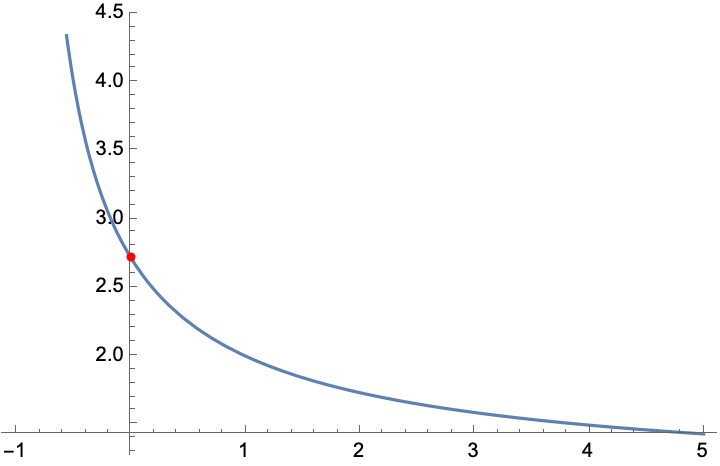
\includegraphics[width=10.0cm]{misc/easalimit.png}
    \caption{Eqn. \ref{eqn:elimit} visualized}
\end{figure}

\section{Linearization}\label{sec:linearization}
\subsection{Linear Approximation}
We can approximate a function by using the equation for its tangent at a particular point.

For example; For a function $y=f(x)$, there exists a point $P = (a, f(a))$. Let $L(x)$ be the line tangent to $f(x)$ at $P$. The slope of $L$ would be defined as:

$$m_L = \frac{\Delta y}{\Delta x} = \frac{L(x) - f(a)}{x - a} = f'(a)$$

Solving for $L(x)$:

\begin{equation}
    \begin{split}
        L(x) - f(a) &= (x-a)f'(a)\\
        L(x) &= f(a) + (x-a)f'(a)\\
    \end{split}
\end{equation}

This function is a fairly good approximation of $f(x)$ near $x=a$, at least for most continuous functions. It's also very important to note that, by definition $f(a) = L(a)$, AND $f'(a) = L'(a)$. This will be expanded upon later.

For example; take $f(x) = sin(x)$, @ $a=0$:

\begin{equation}
    \begin{split}
        f(x) \approx L(x) &= f(\textcolor{red}{0}) + (x-\textcolor{red}{0})f'(0)\\
        &= f(0) + x*cos(0)\\
        &= 0 + x*1\\
        &= x = L(x)
    \end{split}
\end{equation}

\begin{figure}
    \centering
    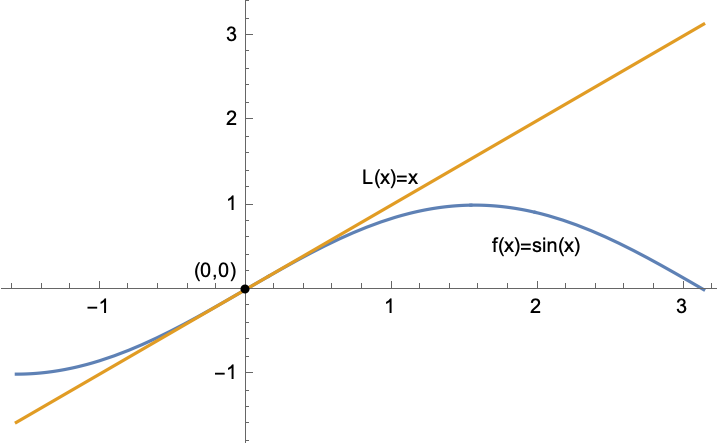
\includegraphics[width=9cm]{misc/linearizationofsinx.png}
    \caption{Linearization of $sin(x)$ at $x=0$}
\end{figure}

Clearly, in the vicinity of $a$, this is a pretty good approximation, but it quickly becomes inaccurate as we move away.

\subsection{Quadratic Approximation}
From the section earlier, we defined $L(x)$, a linear approximation of $f(x)$, where $f(a) = L(a)$ AND $f'(a) = L'(a)$. Now, what if we wanted to continue this trend, and define a new function, $P_2(x)$, where $f(a) = P_2(a)$, $f'(a) = P_2'(a)$, and $f''(a) = P_2''(a)$? Rather than a "linear" approximation, this would, logically, become a "quadratic" approximation. We can say:

\begin{equation}
    \begin{split}
    P_2(x) &= f(a) + (x-a)f'(a) + \textcolor{red}{k(x-a)^2}\\
    P_2(x) &= L(a) + k(x-a)^2\\
    P_2'(x) &= L'(a) + 2k(x-a)\\
    P_2''(a) &= 2k\\
    k &= \frac{P_2''(a)}{2} = \frac{f''(a)}{2}
    \end{split}
\end{equation}

\textit{Note that $L''(a) = 0$; since $L(x)$ is a line, its first derivative is a constant, and its second is 0.}

The purpose of this work was to find some $k$ that we can multiply by a quadratic factor $(x-a)^2$ to maintain the previously stated desired properties of $P_2$. As such, we can rewrite:

$$P_2(x) = f(a) + (x-a)f'(a) + \red{\frac{(x-a)^2}{2}f''(a)}$$

\subsubsection{Taylor Polynomials}
We can, logically, continue this trend for cubic, quartic, etc. approximations. In general, you can approximate any function $f(x)$ to the $N$th power;

$$f(x) \approx P_N(x) = \sum_{n=0}^{N} \frac{(x-a)^n f^{(n)}(a)}{n!}$$

This approximation:
\begin{itemize}
    \item passes through the point $(a,f(a))$
    \item has the same slope, concavity, ..., ie $P_N^{N-1}(a) = f_N^{N-1}(a)$
\end{itemize}

This $N$th degree polynomial is called a \textbf{Taylor Polynomial}, and, intuitively, better approximates $f(x)$ as $N \to \infty$.

When $a = 0$, this polynomial becomes called a \textbf{Maclaurin Polynomial}:

$$P_n(x) = \sum_{n=0}^{N} \frac{x^n f^n(0)}{n!}$$

\subsubsection{Relationship between \texorpdfstring{$f(x)$}{TEXT} and \texorpdfstring{$P_N(x)$}{TEXT}}

While, intuitively, it makes sense that $P_N(x)$ becomes a better approximation of $f(x)$ as $N\to\infty$, this isn't necessarily true.

\textbf{Taylor's Theorem} states the following:

$$f(x) = P_N(x) + R_N(x);$$

where $P_N(x)$ is an approximation (via Taylor Polynomial) of $f(x)$, and $R_N(x)$ is the error in said approximation, defined as:

$$R_N(x) = \frac{(x-a)^{N+1}}{(N+1)!}f^{(N+1)}(c), c \in \real \textit{ and between } x, a$$.

We can then rewrite Taylor's Theorem, as $N$ goes to $\infty$:

$$f(x) = \lim_{N\to\infty}[\sum_{n=0}^N \frac{(x-a)^n f^{N}(a)}{n!} + \frac{(x-a)^{N+1}}{(N+1)!} f^{(N+1)}(c)]$$

Therefore, $f(x) = P_N(x)$ if, and only if, $\lim_{N\to\infty} R_N(x) = 0$. Logically, this should make sense; if there is no remainder, then the approximation is equal to the original function.

\subsection{Taylor Polynomials, Applied Example}\label{sec:taylorcomplex}

Using Taylor Polynomials, we can explore a number of interesting properties of functions, and even derive some unique expressions. For instance (assuming $R_N(x) = 0$):

\begin{equation}\label{eqn:taylorexp}
    \begin{split}
    e^x &= \sum_{n=0}^{\infty} \frac{x^n}{n!} = 1 + x + \frac{x^2}{2!} + ...\\
    e^{\red{i}x} &= 1 + \red{i}x + \frac{(\red{i}x)^2}{2!} + \frac{(\red{i}x)^3}{3!} + ...\\
    e^{\red{i}x} &= 1 -\frac{x^2}{2!} + \frac{x^4}{4!}...+\red{i}[x - \frac{x^3}{3!} + \frac{x^5}{5!}...]\\
    \end{split}
\end{equation}

This may look like it just made things more complicated. However, take a look at the Taylor Polynomial representations of $sin(x)$:

\begin{equation}
    \begin{split}
        f(x) = \sin(x) &= \sum_{n=0}^{\infty} \frac{(x-a)^n f^n(a)}{n!}\\
        f'(x) = \cos(x)\\
        f''(x) = -\sin(x)\\
        f'''(x) = -\cos(x)\\
        f^{IV}(x) = \sin(x)\\
        \therefore f(x) &= 0 + x + 0 + \frac{-x^3}{3!} + 0 + \frac{x^5}{5!} + ...\\
        &= \sum_{n=0}^{\infty}\frac{(-1)^n x^{2n+1}}{(2n+1)!}\\
    \end{split}
\end{equation}

and, very similarly, for $\cos x$:

\begin{equation}
    \begin{split}
        f(x) &= \cos(x) \\
        &= 1 - \frac{x^2}{2!} + \frac{x^4}{4!} + ...\\
        &= \sum_{n=0}^{\infty} \frac{(-1)^n x^{2n}}{(2n)!}
    \end{split}
\end{equation}

Thus, we can rewrite equation \ref{eqn:taylorexp} by substituting in $\sin$ and $\cos$, for the odd and even factors respectively:

\begin{equation}
    \begin{split}
        e^{ix} &= \cos(x) + i\sin(x)
    \end{split}
\end{equation}

This is a very helpful equation, known as \textbf{Euler's Formula}. Some applications are present in Section \ref{complex}.

From here, we can solve for $x=\pi$, to obtain:

\begin{equation}
    \begin{split}
        e^{i\pi} &= \cos(\pi) + i \sin(\pi)\\
        &= -1 + i*0\\
        e^{i\pi}+1 &= 0
    \end{split}
\end{equation}

This ("the most beautiful formula in mathematics") is known as \textbf{Euler's Identity}.

To take this formula further we can solve for $\sin(x)$ and $\cos(x)$ in the imaginary plane. 

\begin{equation}
    \begin{split}
        e^{ix} = \cos(x) + i\sin(x) \implies \cos(x) &= e^{ix} - i\sin(x)\\
        e^{-ix} = \cos(x) - i\sin(x) \implies \cos(x) &= e^{-ix} +i\sin(x)\\
        e^{ix} - i\sin(x) &= e^{-ix} + i\sin(x)\\
        e^{ix}-e^{-ix} &= 2i\sin(x)\\
        \sin(x) &= \frac{e^{ix}-e^{-ix}}{2i}\\
        \cos(x) &= e^{ix}-i\sin(x)\\
        \cos(x) &=e^{ix}-i(\frac{e^{ix}-e^{-ix}}{2i})\\
        \cos(x) &= \frac{e^{ix}+e^{-ix}}{2}\\
    \end{split}
\end{equation}

From here, we can solve for $\cos(ix)$ and $\sin(ix)$:


\begin{equation}
    \begin{split}
        \cos(\red{i}x) &= \frac{e^{i^2 x}+e^{-i(ix)}}{2}\\
        &= \frac{e^x+e^{-x}}{2} = \cosh(x)\\
        \red{i}\sin(x) &= i(\frac{e^{i^2 x}-e^{-i(ix)}}{2})\\
        &= i(\frac{e^x-e^{-x}}{2}) = i \sinh(x)\\
    \end{split}
\end{equation}

And thus, we can define the hyperbolic trigonometric functions using the complex plane, Taylor Series, and Euler's Identity. 

\section{Trigonometry}
% \subsection{Trigonometric Identities}
% There are many, many trigonometric identities that are often (some more than others) useful. See \hyperlink{https://www.overleaf.com/project/633314fad7f84c6632a211a0}{here} for a list of quite a few, accompanied by proofs.
\subsection{Inverse Trig Functions}
As with all functions, we can define the inverse of the basic trig functions, as the functions that undo their respective trig functions. The following shows each of the three basic trig functions, their inverses, and how to derive their respective derivatives.

\begin{itemize}
    \item $y = \arcsin x = sin^{-1}x$
    \begin{equation}
    \begin{split}
        x &= \sin y \\
        \frac{d}{dx}x &= \frac{d}{dx} \sin y\\
        1 &= \frac{d}{dy}[\sin y]\frac{dy}{dx}\\
        1 &= \cos y \frac{dy}{dx}\\
        \frac{dy}{dx} &= \frac{1}{\cos y}\\
        &= \frac{1}{\sqrt{1-\sin^2(y)}} = \frac{1}{\sqrt{1-x^2}}\\
    \end{split}        
\end{equation}

    \item $y = \arccos x = cos^{-1}x$
    \begin{equation}
        \begin{split}
            x &= \cos y\\
            \frac{d}{dx} x &= \frac{d}{dx} \cos y\\
            1 &= \frac{d}{dy}[\cos y] \frac{dy}{dx}\\
            1 &= -\sin y \frac{dy}{dx}\\
            \frac{dy}{dx} &= -\frac{1}{\sin y}\\
            &= -\frac{1}{\sqrt{1-\cos^2(y)}} = -\frac{1}{\sqrt{1-x^2}}
        \end{split}
    \end{equation}

    \item $y = \arctan x = \tan^{-1} x$
    \begin{equation}
        \begin{split}
            x &= \tan y\\
            \ddx x &= \ddx \tan y\\
            1 &= \ddy \tan y \dydx\\
            1 &= \sec^2 y \dydx\\
            \dydx &= \frac{1}{\sec^2 y}\\
            &= \frac{1}{1+\tan^2 y} = \frac{1}{1+x^2}\\
        \end{split}
    \end{equation}
\end{itemize}

\subsection{Hyperbolic Functions}
\subsubsection{Definitions, Identities, Derivatives}
\begin{figure}[!ht]
    \centering
    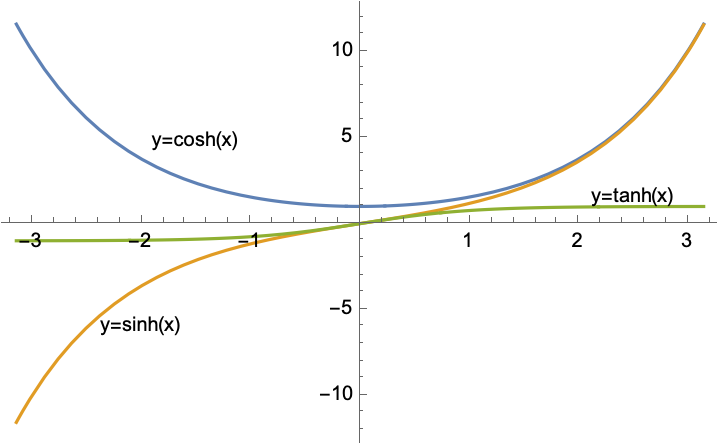
\includegraphics[width=10cm]{misc/coshsinhtanh.png}
    \caption{$\cosh(x), \sinh(x), \tanh(x)$}
    \label{fig:my_label}
\end{figure}
Def:

\begin{equation}
    \begin{split}
        \sinh x &= \frac{e^x-e^{-x}}{2}\\
        \cosh x &= \frac{e^x+e^{-x}}{2}\\
    \end{split}
\end{equation}
Hyperbolic trigonometric functions are the "hyperbolic equivalent" of the basic trig functions. This is an admittedly abstract definition, but there is a more concrete definition in section \ref{sec:taylorcomplex}, using Taylor Polynomials and complex numbers.

The derivatives are as follows; for $\sinh x$:

$$\ddx \sinh x = \ddx [\frac{e^x-e^{-x}}{2}] = \frac{e^x+e^{-x}}{2} = \cosh x;$$

and for $\cosh x$:

$$\ddx \cosh x = \ddx [\frac{e^x+e^{-x}}{2}] = \frac{e^x-e^{-x}}{2} = \sinh x.$$

Note that this is not quite the same relationship between the derivatives of $\sin x$ and $\cos x$.

Similarly, there exist several properties of hyperbolic functions that, while similar in appearance to their equivalent trig functions, have some key differences.

\begin{equation}
    \begin{split}
        \cosh^2 x - \sinh^2 x &= 1\\
        \sinh(x+y) &= \sinh x \cosh y + \cosh x \sinh y\\
        \cosh(x+y) &= \sinh x \sinh y + \cosh x \cosh y\\
    \end{split}
\end{equation}

We can also define $\tanh x$:

$$\tanh x = \frac{\sinh x}{\cosh x} = \frac{\frac{e^x-e^{-x}}{2}}{\frac{e^x+e^{-x}}{2}}=\frac{e^x-e^{-x}}{e^x+e^{-x}};$$

and its derivative:


$$\ddx \tanh x = \ddx [\frac{\sinh x}{\cosh x}] = \frac{\sinh x \sinh x - \cosh x \cosh x}{\cosh^2} = \frac{\sinh^2 x - \cosh^2 x}{\cosh^2 x} = \frac{1}{\cosh^2 x} = sech^2 x.$$

\subsubsection{Inverse Hyperbolic Functions and their Derivatives}

\begin{figure}[!ht]
    \centering
    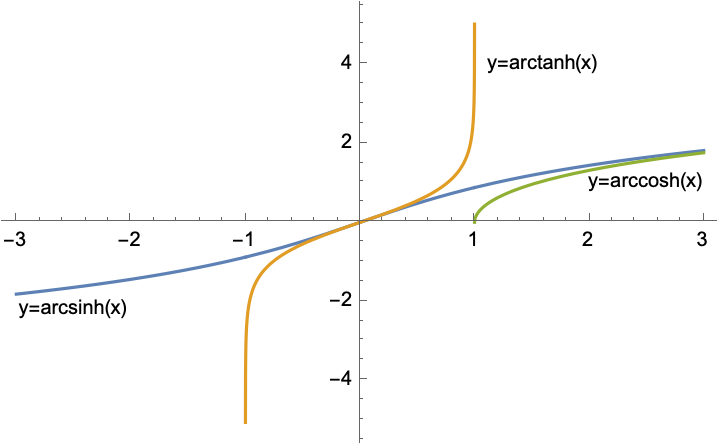
\includegraphics{misc/inversehyperbolic.png}
    \caption{Inverse Hyperbolic Functions}
    \label{inversehyperbolic}
\end{figure}

\begin{equation}
    \begin{split}
        y = \sinh^{-1}(x) \Rightarrow x &= \sinh (y)\\
        \ddx x &= \ddx \sinh(y) \\
        1 &= \dydx \cosh(y)\\
        \dydx &= \frac{1}{\cosh(y)} = \frac{1}{\sqrt{1 + \sinh^2(x)}} = \frac{1}{\sqrt{1+x^2}}\\
        y = \cosh^{-1}(x) \Rightarrow x &= \cosh(y)\\
        \ddx x &= \ddx \cosh(y)\\
        1 &= \dydx \sinh y\\
        \dydx &= \frac{1}{\sinh y} = \frac{1}{\sqrt{cosh^2(y)-1}} = \frac{1}{\sqrt{x^2-1}}\\
        y = \tanh^{-1}(x) \Rightarrow x &= \tanh(y)\\
        \ddx x &= \ddx \tanh(y)\\
        1 &= \ddy \tanh(y) \dydx\\
        1 &= sech^2(y) \dydx\\
        \dydx &= \frac{1}{sech^2(y)} = \frac{1}{1-\tanh^2(y)} = \frac{1}{1-x^2}
    \end{split}
\end{equation}

Note that for $\cosh^{-1}(x)$, the domain of $\cosh(x)$ must be restricted to $x>=0$ so that $\cosh^{-1}(x)$ is a valid one-to-one function. You can see this graphically in figure \ref{inversehyperbolic}.

\subsubsection{Explicitly Expressing Inverse Hyperbolic Functions}

Using the rules of natural logarithms, we can re-express each inverse hyperbolic function explicitly in terms of $x$.

\begin{equation}
    \begin{split}
        y=\sinh^{-1}(x) \Rightarrow x = \sinh y &= \frac{e^y-e^{-y}}{2}\\
        2x &= e^y-e^{-y}\\
        2x\red{e^y} &= (e^y-e^{-y})\red{e^y}\\
        2xe^y &= e^{2y} - 1\\
        0 &= e^{2y} - 2xe^y -1\\
    \end{split}
\end{equation}
This is just a quadratic formula in terms of $e^y$, and can be solved accordingly:

\begin{equation}
    \begin{split}
        e^y &= \frac{2x \pm \sqrt{4x^2+4}}{2}\\
        e^y &= x + \sqrt{x^2+1}\\
    \end{split}
\end{equation}

\textit{We don't take the negative, as $e^y$ is always $>0$}.

\begin{equation}
    \begin{split}
        \ln(e^y) &= \ln(x+\sqrt{x^2+1})\\
        y &= \sinh^{-1}(x) = \ln(x+\sqrt{x^2+1})
    \end{split}
\end{equation}

A very similar process follows for $\cosh$ and $\tanh$, so it won't be shown, but for reference:

\begin{equation}
    \begin{split}
        y &= \cosh^{-1}x = \ln(x+\sqrt{x^2-1})\\
        y &= \tanh^{-1}x = \frac{1}{2} \ln(\frac{1+x}{1-x})
    \end{split}
\end{equation}

\section{Complex Numbers}\label{complex}
\subsection{Complex Quadratic Equations}
To introduce the concept of complex numbers, take an arbitrary quadratic equation of the form 

$$\alpha x^2 + \beta x + \gamma = 0, \alpha, \beta, \gamma \in \mathbb{R}$$.

We can solve this for $x$ as follows:

$$x = \frac{-\beta \pm \sqrt{\beta^2-4\alpha\gamma}}{2\alpha}$$.

If the \textbf{discriminant}, $\beta^2-4\alpha\gamma$, is $<0$, then the equation has no real roots. However, it does have two imaginary roots, of the form

\begin{equation}
    \begin{split}
        x &= \frac{-\beta \pm \sqrt{(-4\alpha)(-\beta^2)}}{2\alpha}\\
        &= \frac{-\beta}{2\alpha} \pm i \frac{\sqrt{4 \alpha \gamma - \beta^2}}{2 \alpha}\\
        &= a \pm  ib; a,b \in \mathbb{R}.
    \end{split}
\end{equation}

This final, simplified form, $a \pm ib$, is also known as "complex conjugates", which has one part ($a$) that is real, and one part ($ib$) that is imaginary. Generally, this is written as $z = a + ib$

\subsection{De Moivre's Formula and Related}

\begin{figure}
    \centering
    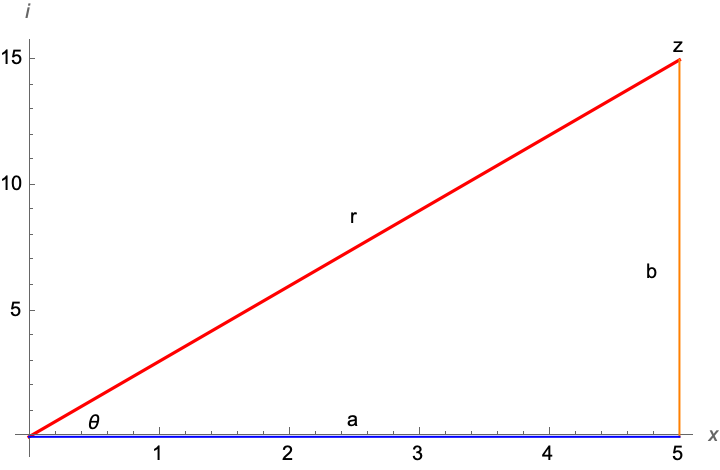
\includegraphics{misc/imaginary.png}
    \caption{The complex plane}
    \label{fig:imaginary}
\end{figure}

Take the equation from the previous section, $z = a + ib$. Figure \ref{fig:imaginary} shows this formula in the complex plane, with $r$ representing the distance between $z$ and the origin $(0,0)$.

\begin{center}
\begin{shaded*}
    \textit{Note that the complex plane is also often referred to as the \textbf{Argand plane}.}
\end{shaded*}
\end{center}

Using this visualization, we can rewrite the formula in the polar form

$$z = r \cos \theta + i r \sin \theta$$.

We can use \textbf{Euler's formula} to simplify this;

\begin{equation}
    \begin{split}
        z &= r(\cos \theta + i \sin \theta)\\
        z &= r e^{i\theta}
    \end{split}
\end{equation}

From this definition, we can define several other properties to aid in solving equations involving complex numbers.

\begin{itemize}
    \item \textbf{Products:} $z_1z_2 = r_1 e^{i\theta_1} r_2 e^{i\theta_2} = r_1 r_2 e^{i(\theta_1+\theta_2)}$
    \item \textbf{Quotients:} $\frac{z_1}{z_2} = \frac{r_1}{r_2} e^{i(\theta_1-\theta_2)}$
    \item \textbf{Powers:} $z^n = r^n e^{i n \theta}, n \in \integers$
\end{itemize}

Example: calculate $(-1-i)^{20}$. See figure \ref{fig:demoivreseg} for a visual representation.

\begin{figure}[!ht]
    \centering
    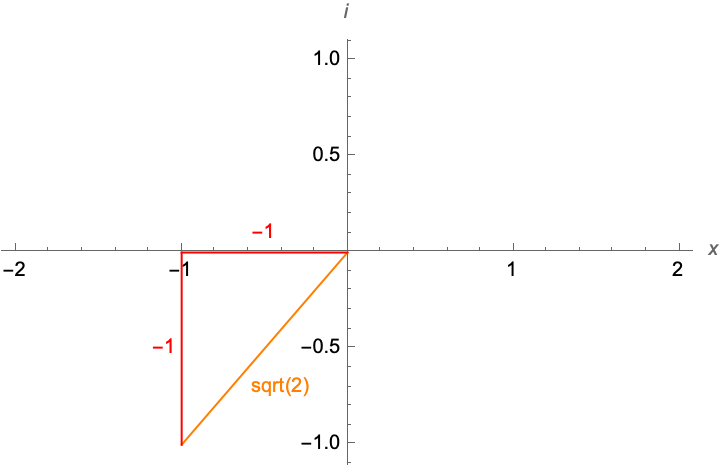
\includegraphics[width=8cm]{misc/demoivresexample.png}
    \caption{$(-1-i)$ represented on the complex plane}
    \label{fig:demoivreseg}
\end{figure}

\begin{equation}
    \begin{split}
        (-1-i)^{20} = z^n &= r^n e^{i n \theta}\\
        &= \red{\sqrt(2)}^{20} e^{i 20 * \frac{5\pi}{4}}\\
        &= 2^{10} e^{25 \pi i }\\
        &= 1024 e^{24 \pi i} e^{\pi i}\\
        &= 1024 * (1) (-1) \\
        &= -1024
    \end{split}
\end{equation}

Note that the second to last step is done using Euler's Identity; specifically:
\begin{equation}
    \begin{split}
        e^{i \pi} &= -1\\
        e^{n i\pi} &= e^{{(i\pi)}^{n}}= -1^{n}, n \in \integers\\
        n &= \{0, 2, 4, ...\}, e^{n i \pi} = 1\\
        n &= \{1, 3, 5, ...\}, e^{n i \pi} = -1\\
    \end{split}
\end{equation}

\subsubsection{Roots}

We can use some of the identities above to find a formula to find the real AND complex roots of number:

\begin{equation}
    \begin{split}
        z &= r e^{i \theta} = re^{i(\theta +2k\pi)}, k \in \integers \ge 0\\
        z^{\frac{1}{n}} &= z^{\frac{1}{n}}e^{\frac{i (\theta + 2k\pi}{n}}, k = 0,1,..(n-1)\\
    \end{split}
\end{equation}

For example, to find all of the cube roots of 8:

\begin{equation}
    \begin{split}
        z &= 8 = 8e^{2k\pi i}\\
        z^{\frac{1}{3}} &= 8^{\frac{1}{3}} = 8^{\frac{1}{3}}e^{\frac{2k\pi i}{3}}, k = 0,1,2\\
        &z_{k=0} = 8^{\frac{1}{3}}e^{0} = 2\\
        &z_{k=1} = 8^{\frac{1}{3}}e^{\frac{2\pi i}{3}} = 2e^{\frac{2\pi}{3}}=2[cos\frac{2\pi}{3}+i\sin\frac{2\pi}{3}] = 2[-\frac{1}{2}+i\frac{\sqrt(3)}{2}] = -1 + i \sqrt{3}\\
        &z_{k=2} = 8^{\frac{1}{3}}e^{\frac{4\pi i}{3}} = ... = -1 - i \sqrt{3}
    \end{split}
\end{equation}

Thus, the cube roots of 8 are $2, -1 + i\sqrt{3}, -1 - i\sqrt{3}$.

Another method of solving for the roots of a complex number (which can also be extended to other problems involving complex numbers, but is most obvious when calculating roots) involves a little more intuition rather than just using the polar form immediately. 

Say you are solving for the square roots of $-8-15i$, ie $(-8-15i)^\frac{1}{2}$. We can then say:

\begin{equation}
    \begin{split}
        (-8-15i)^\frac{1}{2} &= a + bi, a, b\in \real\\
        -8-15i &= (a + bi)^2 = a^2+2abi-b^2 = a^2-b^2+2abi\\
        &\Rightarrow-8 = a^2-b^2\\
        &\Rightarrow-15 = 2ab\\
    \end{split}
\end{equation}

Logically, the roots of a complex number involve some real part ($a$) and some imaginary part ($bi$). Using this knowledge, we can use the above steps to find $a$ and $b$ using more basic algebra. Doing the work out fully will result in a quadratic formula for $a$ and $b$, which can finally be solved for the values of the roots (the $\pm$ in the quadratic formula allows for the creation of two roots).

\subsubsection{Logarithms}

We can use some of the identities above to also find a log involving complex numbers:

\begin{equation}
    \begin{split}
        z &= re^{i\theta}\\
        \ln(z) &= \ln(re^{i\theta})\\
        &= \ln(r) + \ln(e^{i\theta})\\
        &= \ln(r) + i\theta
    \end{split}
\end{equation}

For example, to find $\ln(-1)$:

\begin{equation}
    \begin{split}
        \ln(-1) &= \ln(1) + i(\pi + 2n\pi)\\
        &= i(\pi + 2n\pi), n = 0, \pm 1, \pm 2, ...\\
    \end{split}
\end{equation}

\section{Applications of Differentiation}
\subsection{Related Rates}

"Related rates" problems are very common, and often follow very similar patterns that can be exploited to make individual problems very straightforward. Generally:

\begin{enumerate}
    \item Draw a picture to represent the scenario
    \item Write a formula involving the variable whose change is given, in relation to the variable whose change you're solving for
    \begin{enumerate}
        \item Many times, said formula will have to be simplified/rewritten in terms of a single variable. This often involves similar triangles in geometric questions.
    \end{enumerate}
    \item Differentiate, then solve accordingly
    \begin{enumerate}
        \item This pretty much always involves implicit differentiation
    \end{enumerate}
\end{enumerate}

The best way to approach these questions is to simply practice. The patterns between questions will quickly become obvious.
\subsection{Rolle's Theorem}
\begin{figure}[!ht]
    \centering
    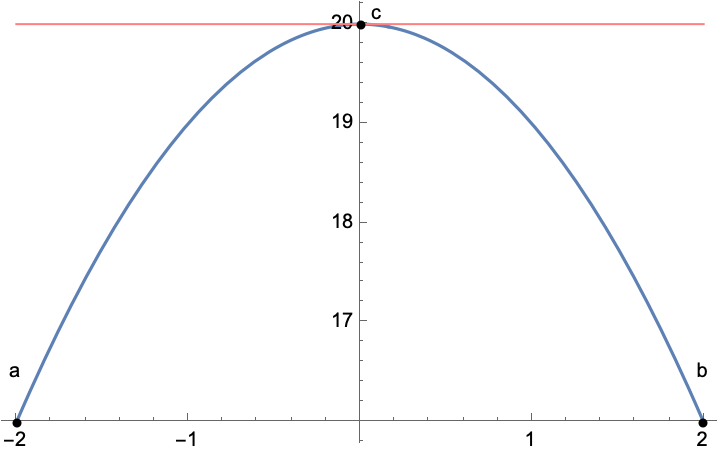
\includegraphics[width=9cm]{misc/rolles.png}
    \caption{Rolle's Theorem visualized}
    \label{fig:rolles}
\end{figure}
\begin{shaded}
If a function $f$
\begin{itemize}
    \item is \textit{continuous} on $[a,b]$
    \item is \textit{differentiable} on $(a,b)$
    \item $f(a) = f(b)$
\end{itemize}
then there is a number $c$ in $(a,b)$ such that $f'(c) = 0$.
\end{shaded}

The proof for this theorem is fairly straightforward (and intuitive), and also makes a lot of sense graphically (see figure \ref{fig:rolles}).

\subsection{Mean Value Theorem}
\begin{figure}[!ht]
    \centering
    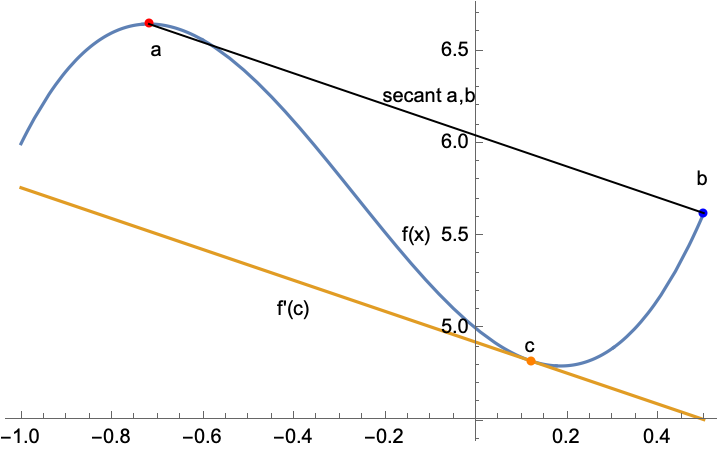
\includegraphics[width=10cm]{misc/mvt.png}
    \caption{The Mean Value Theorem visualized}
    \label{fig:mvt}
\end{figure}
\begin{shaded}
    If a function $f$ is
    \begin{itemize}
        \item \textit{continuous} on $[a,b]$
        \item \textit{differentiable} on $(a,b)$
    \end{itemize}
    then there exists a $c$ in $(a,b)$ such that $\frac{f(b)-f(a)}{b-a} = f'(c)$. See figure \ref{fig:mvt}.
\end{shaded}

This theorem is essentially an application of Rolle's Theorem, but for any $a,b$ that are not necessarily equal. The "official" proof for this theorem is fairly straightforward as well, but again, is fairly intuitive graphically.

This, and Rolle's, are useful in questions involving proving the number of roots in an equation, as well as proving other theorems.

\subsection{Optimization}
Optimization questions are (\textit{at least to me}) very similar to related rates questions. In both, you have to find some sort of formula representing a situation, then differentiating. However, for optimization questions, the intention is to solve for a min/max value, by finding when the derivative ("rate of change") is 0. Logically this should make a lot of sense: when something is not changing ($\dxdy = 0$), then it has to be either increasing until that point and then begin to decrease, or vice versa. From here, checking the second derivative will reveal whether it was a min or max. 

In many situations, you will have to ensure that your min/max fits within some endpoints, which depend on the situation at hand; eg, if you have a geometric question, then your value logically can't be negative. 

\textbf{A summary of general steps:}
\begin{itemize}
    \item Draw a diagram, assign relevant variables, create a formula
    \item Differentiate the formula, set it equal to 0, and solve for the unknown(s) that satisfy the question
    \item Check the sign of the second derivative of the formula to ensure that your value really was a min/max
    \item Check the "endpoints" of the problem (are either logical, or imposed by the wording in the question), and ensure that your min/max falls within that range
    \begin{itemize}
        \item If it doesn't, this usually means your ACTUAL min/max is one of the endpoints, so be careful for this
    \end{itemize}
\end{itemize}
\subsection{Error and Uncertainty}
\subsubsection{Uncertainty}
\begin{figure}[!ht]
    \centering
    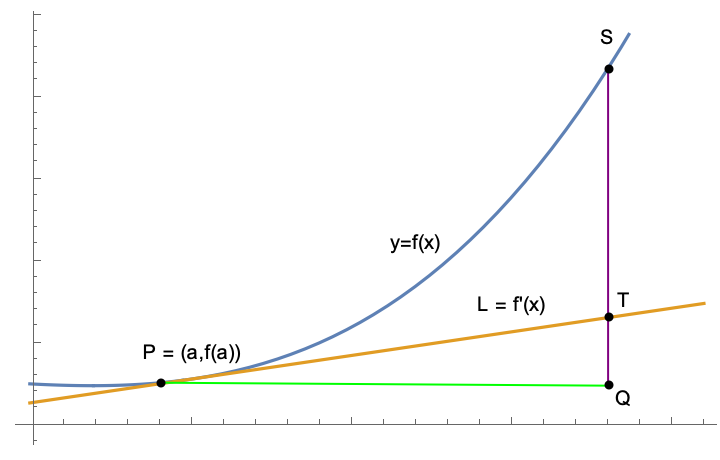
\includegraphics[width=9cm]{misc/differentialserrors.png}
    \caption{Visual representation of using a differential to approximate error}
    \label{fig:dxtoapproxerrors}
\end{figure}

One very helpful use of derivatives is in estimating how some variable changes when given the relative change in another. This same idea is very similar to the rationale behind using differentials to estimate an error in a measurement, but this will be further explained a little later.

To show how a derivative of a function at a point can be used to estimate its change over a particular range, consider a function $y=f(x)$, as shown in figure \ref{fig:dxtoapproxerrors}.

As discussed in \ref{sec:linearization}, we can define $L$ as the linear approximation of $f(x)$ at $P$ as $L = f(a) + (x-a)f'(a)$

As shown in the graph, $PQ = \Delta x = dx$; note that this is the change in $x$ of both $f(x)$ AND $L$. Conversely, $QS = \Delta y$, the change in $f(x)$, and $QT = dy$, the change in $L$. In summary:

\begin{equation}
    \begin{split}
     L &= f(a) + (x-a)f'(a)\\
     PQ &= \Delta x = dx\\
     QS &= \Delta (f(x)) = \Delta y\\
     QT &= \Delta (L(x)) = dy
    \end{split}
\end{equation}

From here, we can define $\theta$ as the angle between $PQ$ and $PT$. As such:

\begin{equation}
    \begin{split}
        \frac{QT}{PQ} &= \tan \theta = f'(a)\\
        &\therefore QT = f'(a)PQ\\
        dy &= f'(a)\Delta x =  f'(a) dx\\
        &\therefore QS \approx QT \therefore \Delta y \approx dy = f'(a) \Delta x = f'(a) dx
    \end{split}
\end{equation}

As shown, $dy$ is a good approximation for $\Delta y$ when $\Delta x$ is relatively small. This reasoning can also be applied to the logic behind why a linear approximation $L(x)$ of a function $f(x)$ at $a$ is most accurate when $x \approx a$.

\textbf{For example:} say you were asked to find $\cos(\frac{\pi}{3}+0.05)$. In this case, we can say $f(x) = \cos(x)$, $a = \frac{\pi}{3}$, and $\Delta x = dx = 0.05$. From here:

\begin{equation}
    \begin{split}
        f'(x) &= -\sin(x)\\
        f'(a) &= -\sin(\frac{\pi}{3}) = -\frac{\sqrt{3}}{2}\\
        dy &\approx f'(a)dx = \frac{-\sqrt{3}}{2}*0.05 \approx -0.043
    \end{split}
\end{equation}

In reality, $\cos(\frac{\pi}{3}+0.05) = -0.044$, demonstrating how accurate (and easy-to-compute) this method is.

\subsubsection{Error}
Using very similar reasoning to above, we can use differentials to find the range of error in a calculation. If given the error (change) of one variable in a formula, you can then use implicit differentiation, and solve for the error (change) in the desired variable.

Oftentimes, "relative change" is also asked for. This is simple $\frac{dx}{x}$.

\textbf{For example:} given a circle with radius $r=24$, with a max error in measurement of $0.2$. To find the max error in the circle's area:

\begin{equation}
    \begin{split}
        A &= \pi r^2 = f(r)\\
        \Delta A &\approx dA = f'(r) dr\\
        &= 2\pi r dr\\
        &= 2\pi(24)(0.2) = 9.6 \pi \approx 30.16\\
        &\textit{rel. error:} \frac{\Delta A}{A} \approx \frac{dA}{A} = \frac{1}{60}
    \end{split}
\end{equation}
\subsection{Newton's Method}
\textbf{Newton's Method} is an application of derivatives that can be used to estimate the solutions/roots of a function. The steps to the method are as follows, for a function $f(x)$:

\begin{enumerate}
    \item Pick some $x_1$, then find the point $P = (x_1, f(x_1))$
    \item Find the tangent line of $f(x)$ at the point $P$, defined by $y - f(x_1) = f'(x_1)(x-x_1)$
    \item Find the point $x_2$ where the tangent line intersects the $x$-axis, by setting $y=0$: 
    \begin{equation}
        \begin{split}
            0 &= f(x_1)+f'(x_1)(x_2-x_1)\\
            x_2 &= x_1 - \frac{f(x_1)}{f'(x_1)}\\
        \end{split}
    \end{equation}
    
    \item Repeat steps 1-3 for increasing $x_n$ and $x_{n+1}$. As $n$ increases, the $x_n$ will approach a root of $f(x)$. The general formula follows:
    
    $$x_{n+1} = x_{n} - \frac{f(x_n)}{f'(x_n)}$$
    
    See figure \ref{fig:newtonsmethod} to see this process visually.
\end{enumerate}

\begin{figure}[!ht]
    \centering
    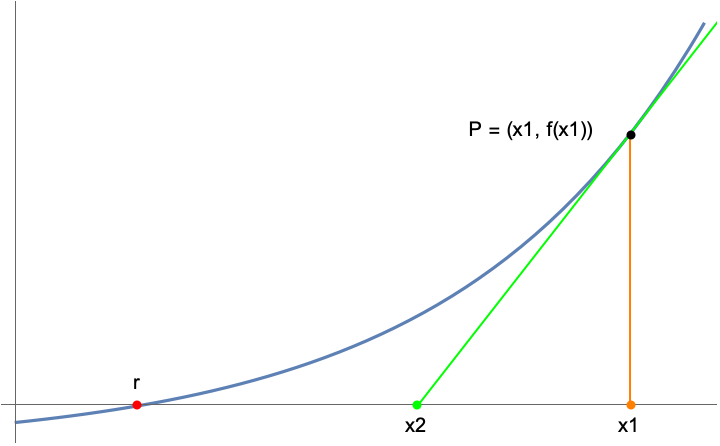
\includegraphics[width=9cm]{misc/newtonsmethod.png}
    \caption{Newton's Method Visualized}
    \label{fig:newtonsmethod}
\end{figure}

\subsection{Derivative-Related Theorems}

Following are a number of theorems related to derivatives, and limits. While many of them are already described above, some are not.

These theorems have various applications in determining limits and derivatives and can aid in graphing functions.

\begin{enumerate}
    \item \textbf{Intermediate Value Theorem}
    
    If $f$ is continuous on $[a,b]$, let $N$ be any number between $f(a)$ and $f(b)$, where $f(a) \neq f(b)$, there exists a $c$ in $(a,b)$ such that $f(c) = N$.
    
    \item \textbf{Extreme Value Theorem}
    
    If $f$ is continuous on $[a,b]$, then $f$ attains a minimum and maximum value (extrema) on that interval. 
    \textit{Not that these extrema may occur at $a$ or $b$; make sure to check this case when answering questions using this theorem.}
    
    \item \textbf{Fermat's Theorem}
    
    If $f$ has a local extrema at $c$, and $f'(c)$ exists, then $f'(c) = 0$. 
    
    \textit{Note that the inverse of this theorem is not necessarily true: if $f'(b) = 0$, then $b$ is not necessarily a local extrema.}
    
    \item \textbf{Rolle's Theorem}
    
    If $f$ is continuous on $[a,b]$, $f'$ is continuous on $(a,b)$, and $f(a) = f(b)$, then there exists a $c$ in $(a,b)$ such that $f'(c) = 0$.
\end{enumerate}

\subsection{Graph Sketching}

Using calculus (and other properties of functions), we can sketch curves with fairly high accuracy, without needing calculators. To do so, there is a "shopping list" to follow, to graph a function $f(x)$:

\begin{enumerate}
    \item \textbf{Domain}
    
     Find all $x$ for which $f(x)$ is defined. If $f(x)$ is undefined for some $x$, you should also find how $f$ behaves as it approaches $x$ (is it a hole? An asymptote? Or does the function simply only exist on a closed interval?)
     
    \item \textbf{Intercepts}
    
    Find both the $x$ and $y$ intercepts, i.e. the ordered pair $(x,f(x))$ at $y=0$ and $x=0$ respectively.
    
    \item \textbf{Symmetry (even/odd)}
    \begin{itemize}
        \item $f(x) = f(-x)$: $f(x)$ is \textbf{even}
        \item $f(-x) = -f(x)$: $f(x)$ is \textbf{odd}
    \end{itemize}
    
    Graphically, an even function is symmetrical over the $y$ axis, and an odd function is symmetrical over $y=x$.
    
    \item \textbf{Asymptotes}
    
    Determine $\lim_{x\to\infty} f(x)$ and $\lim_{x\to-\infty}$, to determine whether the function has any \textbf{horizontal asymptotes}. In addition, find the limit of $f(x)$ to any holes in the domain, from both right and left, to determine if the function has any \textbf{vertical asymptotes}. 
    
    \item \textbf{Intervals of Increase/Decrease \& Local Min/Max}
    
    Find $f'(x)$, and find when $f'(x)$ is greater/less than 0 to find when $f(x)$ is increasing/decreasing respectively. The points where $f'(x) = 0$ are also the place where the function has a local min/max, AS LONG AS $f'(x)$ is not an inflection point...
    
    \item \textbf{Concavity \& Points of Inflection}
    
    Find $f''(x)$, and find when $f''(x)$ is greater/less than 0 to find when $f(x)$ is concave up/down respectively. The points where $f''(x) = 0$ are also the inflection points of $f(x)$.
\end{enumerate}

\section{Integration}
\subsection{Defining Antiderivatives}

For a function $f(x)$, we can say that:

$$\int f(x) dx = F(x) + k$$,

where $\ddx [F(x)+k] = f(x)$, and $k$ is a constant.

For example: $\int x^2 dx = \frac{x^3}{3} + k$.

You can (and should) think of $\int  dx$ and $\ddx$ as \textit{inverse operators} of one another, hence the term "antiderivative". As such, numerous derivative rules have corresponding rules for integrals, which are discussed later. Also note that this type of integration is called \textit{indefinite} because it defines the integral of a function over an \textit{indefinite range}, ie, for all $x$. \textit{Definite integrals} will be discussed later and have their own very particular applications, and define an integral $\int_m^n$ over a range $[m,n]$.

\subsection{Techniques of Integration}
\subsubsection{Known Formulas of Derivatives}

eg) $\int \frac{1}{1+x^2} dx = \arctan x + c$

"Simply" recognize that the integral to solve for is the derivative of a common function. Most other techniques of integration involve simplifying/modifying a given integral into this type of easy-to-solve form.

\subsubsection{By Substitution}

For many integrals, we can substitute part of a complex expression for a single variable (typically $u$; this technique is often shorthanded "$u$-sub"), and, following some manipulation, find an integral much more easily. The best way to understand this method is through an example:

$$\int \sqrt{x^3+2}x^2 dx$$

We can let $u = x^3+2$, and differentiating $u$ in terms of $x$, we get

\begin{equation}
\begin{split}
    \frac{du}{dx} &= 3x^2\\
    du &= 3x^2 dx\\
    x^2 dx = \frac{du}{3}\\
    \end{split}
\end{equation}

From here, we can substitute our expressions back into the original integral, and solve:

\begin{equation}
    \begin{split}
    \int \sqrt{x^3+2}x^2 dx &= \int u^\frac{1}{2} \frac{du}{3}\\
    &= \frac{1}{3} \frac{u^{\frac{3}{2}}}{\frac{3}{2}} + k\\
    &= \frac{2(x^3+2)^{\frac{3}{2}}}{9} + k\\
    \end{split}
\end{equation}

Note that solving this integral involved using the inverse of the "power rule" of derivatives, which should hopefully be intuitive.

\subsubsection{By Parts}

Given two functions $u$ and $v$, we can write:

\begin{equation}
\begin{split}
    \frac{d}{dx}[uv] &= \frac{du}{dx} v + u \frac{dv}{dx}\\
    \int (\frac{d}{dx}[uv] &= \frac{du}{dx} v + u \frac{dv}{dx})dx\\
    \int \frac{d}{dx} [uv] dx &= \int [v \frac{du}{dx}] dx + \int [u \frac{dv}{dx}] dx\\
    uv &= \int v du + \int u dv\\
    \int u dv &= uv - \int v du\\
\end{split}
\end{equation}

For example, to calculate the integral of $x e^{ax}$:

\begin{equation}
    \begin{split}
        \int x e^{ax} dx&\\
        x &= u, du = dx\\
    e^{ax} dx &= dv, v = \frac{e^{ax}}{a}\\
    &\int x e^{ax} dx = x \frac{e^{ax}}{a} - \int \frac{e^{ax}}{a} dx\\
    &= \frac{xe^{ax}}{a} - \frac{e^{ax}}{a^2}+C\\
    \end{split}
\end{equation}

Generally, you want to find some $u$ such that $du$ becomes "simpler", and a $dv$ such that $v$ does not get "too much more complicated".

Another integral that is commonly computed using integration by parts is as follows:

\begin{equation}
    \begin{split}
        \int \ln x dx&\\
        &= x \ln x - \int x \frac{dx}{x}\\
        &= x \ln x - x + C
    \end{split}
\end{equation}

\subsubsection{Trigonometric Integrals}

Finding the integral of a combination of trigonometric functions is largely a question of using trig. identities in such a way that the integral becomes easier to solve using more "basic" methods. 

While a lot of this becomes intuitive over time, some general guidelines are as follows:

\begin{itemize}
    \item $\int \sin^m(x)\cos^n(x) dx$
    
    If \textbf{$n$ is odd ($n=2k+1$)}, rewrite all $\cos$, except one, with $\cos^2(x)=1-\sin^2(x)$.
        
        \begin{equation}
            \begin{split}
                \int \sin^{m}(x) \cos^{2k+1}(x) dx &= \int \sin^m(x)(\cos^2x)^k\cos(x) dx\\
                &= \int \sin^m(x)(1-\sin^2(x))^k\cos(x) dx
            \end{split}
        \end{equation}
        
        From here, substitute $u=\sin(x)$ and solve accordingly.
        
        Very similarly, \textbf{if $m$ is odd ($m=2k+1$)}:
        
        \begin{equation}
            \begin{split}
                \int \sin^{2k+1}(x) \cos^{n}(x) dx &= \int (\sin^2(x))^k \cos^n(x) \sin(x) dx\\
                &= \int (1-\cos^2x)^k\cos^n(x)\sin^n(x) dx
            \end{split}
        \end{equation}
        
        Let $u = \cos(x)$, etc..

        \textbf{If both $m$ and $n$ are even}, you can use the half-angle theorems.
        
    \item $\int \tan^m(x)\sec^n(x) dx$
    
    Very similar to the strategy for $\sin$ and $\cos$: if $n$ is even, substitute $\sec^2(x) = 1+\tan^2(x)$ for all $\sec$ except one, and the opposite for $\tan^2(x)$ if $m$ is even.
\end{itemize}

\subsubsection{Trigonometric Substitution}

Using a strategy similar to "u-substitution", we can carefully replace variables in an integral with trigonometric functions to make the integral easier to solve.

In general, we can say:

$$
\int f(x) dx = \int f(g(t)) g'(t) dt
$$

There are three main forms to look out for in integrals that can be used to effectively substitute trigonometric functions. Notice that, in each case, a form similar to a common trigonometric identity is present.

\begin{itemize}
    \item $\sqrt{a^2-x^2}  \Rightarrow x = a \sin \theta $ 
    
    \item $\sqrt{a^2+x^2} \Rightarrow x = a \tan \theta$
    
    \item $\sqrt{x^2-a^2} \Rightarrow x = a \sec \theta$
\end{itemize}

Using this strategy makes a lot more sense when used in an example; say $\int \frac{\sqrt{9-x^2}}{x^2} dx$. This is of the first form listed above, so we can substitute $x=3\sin \theta$, meaning $dx = 3\cos\theta d\theta$. Assume $-\frac{\pi}{2} \leq \theta \leq \frac{\pi}{2}$

\begin{equation}
    \begin{split}
        \int \frac{\sqrt{9-x^2}}{x^2}dx &= \int \frac{\sqrt{9-9\sin^2(\theta)}}{9\sin^2(\theta)}3\cos(\theta)d\theta\\
        &= \int \frac{\sqrt{9\cos^2(\theta)}}{9\sin^2(\theta)}3\cos(\theta)d\theta\\
        &= \int \frac{3\cos(\theta)}{9\sin^2(\theta)}3\cos(\theta)d\theta\\
        &= \int \frac{\cos^2)(\theta)}{\sin^2(\theta)}d\theta = \int \cot^2(\theta) d\theta\\
        &= \int (\csc^2(\theta)-1)d\theta = -\cot(\theta) -\theta + C
    \end{split}
\end{equation}

From here, the integral can be rewritten in terms of $x$ using some trig rules (drawing a diagram of a triangle can help here):

$$-cot(\theta)-\theta + C = -\frac{\sqrt{9-x^2}}{x}-\sin^{-1}(\frac{x}{3})+C$$
\subsection{Applications of Integrals}

\section{Differential Equations}
\subsection{Definitions}

A \textbf{differential equation} is an equation that contains an unknown function and some of its derivatives. We can more specifically describe differential equations by their \textbf{order}, which is the number of the highest derivative in the equation, ie, a first-order differential equation is of the form $F(x,y,y')$.

\subsection{Variables Separable}\label{sec:separable}

While not all differential equations are solvable (or at least, easily solvable), one (of many) special cases is of the form:

\[
\dydx = f(x)g(y) = \frac{f(x)}{h(y)}, g(y) = \frac{1}{h(y)}, h(y) \neq 0
\]

This is the form of a function of $x$ times a function of $y$, indicating the parts are \textit{separable}. We can rewrite this:

\begin{equation}
    \begin{split}
        \dydx &= f(x)g(y)\\
        dy &= [\frac{dy}{dx}]dx = f(x)g(y)dx\\
        \int \frac{dy}{g(y)} &= \int \frac{dx}{f(x)}
    \end{split}
\end{equation}

From here, integrating both sides yields either $y$ as a function of $x$, or $x$ as a function of $y$ (which one you solve for depends on the context of the question).

For example, take: $\frac{dy}{dx} = x^2 y - y + x^2 -1$. This can be rewritten as a separable equation:

\begin{equation}
    \begin{split}
        \frac{dy}{dx} &= x^2y-y+x^2-1\\
        &= y(x^2-1)+1(x^2-1)\\
        &= (y+1)(x^2-1)\\
        \int \frac{dy}{y+1} &= \int (x^2-1)dx\\
        \ln(|y+1|) &= \frac{x^3}{3} - x + k\\
        y + 1 &= \pm e^{(\frac{x^3}{3}-x+k)} = \pm e^{(\frac{x^3}{3}-x)}e^k\\
        y &= Ce^{(\frac{x^3}{3}-x)}-1, C = \pm e^k
    \end{split}
\end{equation}

From here, if given $y(0)$, you can solve for the value of $C$ and rewrite the equation appropriately. This would then become what is called an \textbf{initial value problem} (IVP); you are given the initial value, after all. 

In this example, say $y(0) = 3$. We can write:

\begin{equation}
    \begin{split}
        3 &= Ce^{\frac{(0)^3}{3}-0}-1\\
        3 &= Ce^0-1\\
        C &= 4\\
        y = 4e^{\frac{x^3}{3}-x}-1\\
    \end{split}
\end{equation}

\subsection{Mathematical Models}

% wtf does this mean? rewrite...
Several real-world scenarios can be represented using differential equations, and the following are some of the more common/useful forms, as well as their general solutions and applications.

\begin{itemize}
    \item[\textbf{I:}] $\alpha y = \frac{dy}{dt}, \alpha \in \real$ 
    
    When solved for a function $y$ of $t$, this differential equation becomes a (hopefully) familiar form;
    
    \begin{equation}
        \begin{split}
            \frac{dy}{dt} &= \alpha y\\
            \int \frac{dy}{y} &= \int \alpha dt\\
            \ln|y|&=\alpha t + C\\
            y &= \pm e^{(\alpha t + C)} = \pm e^C e^{\alpha t} = k e^{\alpha t}, k = \pm e^C\\
        \end{split}
    \end{equation}
    
    If we say $y(0) = y_0$, then we can rewrite $y(t)=y_0e^{\alpha t}$. This is the typical form used to represent simple \textbf{exponential growth/decay}; which of these two the function represents depends on $\alpha$:
    
    \begin{itemize}
        \item $\alpha > 0$;\textbf{growth:} used in scenarios such as simple population models.
        \item $\alpha < 0$; \textbf{decay:} used in scenarios such as radioactive decay.
    \end{itemize}
    
    See figure \ref{fig:exponentialgrowthndecay} for a visual representation of these two.
    
    \begin{figure}[!ht]
        \centering
        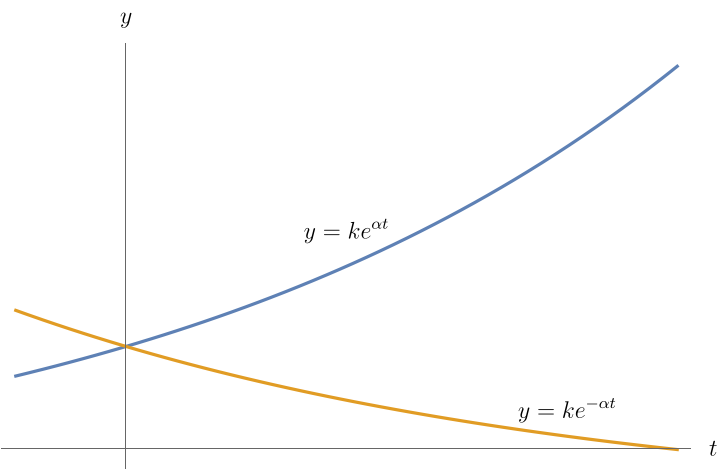
\includegraphics[width=9.6cm]{misc/exponentialgnd.png}
        \caption{Exponential growth and decay}
        \label{fig:exponentialgrowthndecay}%
    \end{figure}
    
    \item[\textbf{II:}] $\frac{dy}{dt} = k(N-y)$ 
    
    This general form of the equation is used in a number of scenarios, such as Newton's Law of cooling/heating and modeling deprecation. Solving this differential for $y$ as a function of $t$ goes as follows:
    
    \begin{equation}
        \begin{split}
            \frac{dy}{dt} &= k(N-y)\\
            \frac{dy}{N-y} &= k dt  \\
            \int \frac{dy}{N-y} &= \int k dt\\
            - \ln|N-y| &= kt + C\\
            N-y &= \pm e^{-C}e^{-kt} = Ke^{-kt}\\
            y &= N-Ke^{-kt}\\
        \end{split}
    \end{equation}
    
    If we state that $y(0) = y_0$, we can rewrite this equation as $y = N+(y_0-N)e^{-kt}$. This is the same form that Newton's Law of Cooling takes: $T(t) = T_{env} + (T(0) - T_{env})e^{-rt}$.
    
    It's important to note that $y(t)$ approaches $N$ as time approaches infinity, ie:
    
    $$\lim_{t\to\infty} [N+(y_0-N)e^{-kt}] = N$$
    
    If the value of $y_0-N$ is positive, then this limit is approached from above (ie, the function is \textit{lower bounded} by $N$), and if $y_0-N$ is negative, then the limit is approached from below (\textit{upper bounded} by $N$). See figure \ref{fig:newtonscooling} for a visual representation of the difference, assuming a constant $y_0$.
    
    \begin{figure}[!ht]
        \centering
        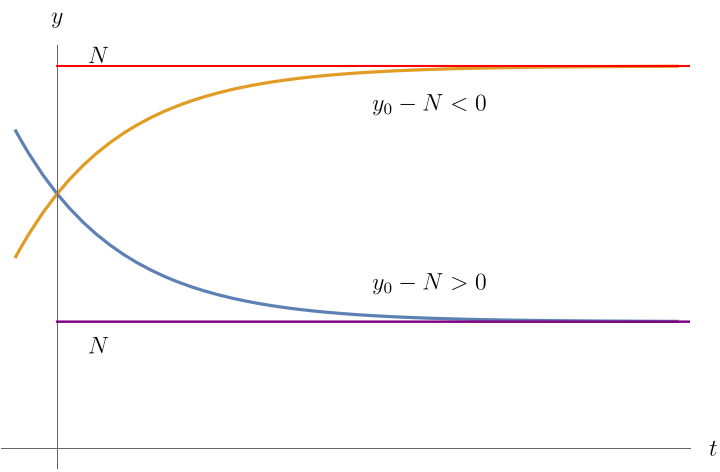
\includegraphics[width=9.6cm]{misc/newtonscooling.png}
        \caption{$y=N+(y_0-N)e^{-kt}, y_0-N > 0$ vs $y_0-N < 0$}
        \label{fig:newtonscooling}
    \end{figure}
    
    \item[\textbf{III:}] $\frac{dy}{dt} = \frac{k}{N}y(N-y)$
    
    This differential equation represents a general form of the \textbf{logistic equation}, commonly used in population modeling in ecology and other fields. Solving this differential equation for $y$ as a function of $x$ goes as follows:
    % this is all wrong
    \begin{equation}
        \begin{split}
            \frac{dy}{dt} &= \frac{k}{N}y(N-y)\\
            \frac{dy}{y(N-y)} &= \frac{k dt}{N}\\
            \int \frac{dy}{y(N-y)} &= \int \frac{k dt}{N}\\
            \int [\frac{\frac{1}{N}}{y} + \frac{\frac{1}{N}}{N-y}] dy &= \frac{k}{N} t + C\\
            \frac{1}{N}(\ln|y| - ln|N-y|) &= \frac{k}{N} t + C\\
            \ln|\frac{y}{N-y}| &= kt + D, D = CN\\
            \frac{y}{N-y} &= Ke^{kt}, K = \pm e^D\\
            y &= \frac{NKe^{kt}}{1+Ke^{tx}} =\frac{NKe^{kt}}{1+Ke^{kt}} \frac{\frac{e^{-kt}}{K}}{\frac{e^{-kt}}{K}}\\
            &= \frac{N}{\frac{e^{-kt}}{K} + 1} = \frac{N}{1+be^{-kt}}, b = \frac{1}{K}\\
        \end{split}
    \end{equation}

    If we say $y(0) = P_0$, or the initial population, then we can simplify further and say:

    \begin{equation}
        \begin{split}
            y(0) = P_0 &= \frac{N}{1+b}\\
            \implies b &= \frac{N}{P_0} - 1 = \frac{N-P_0}{P_0}\\
            \therefore y(t) &= \frac{N}{1+be^{-kt}}, b = \frac{N-P_0}{P_0}\\
            y(t) &= \frac{NP_0}{P_0 + (N-P_0)e^{-kt}}\\
        \end{split}
    \end{equation}

    Just as with Model II, the function approaches $N$ as the time goes to infinity, and as such, we can call $N$ the "carrying capacity" or "max population", depending on the context of the problem.

    Another interesting property of the logistic model comes about from exploring its derivatives. Its first derivative is clear, as it is given in the expression of the logistic model as a differential equation. This first derivative ($\frac{dy}{dt}$) is \textit{always positive}, which should be clear from inspection of the original formula for $\frac{dy}{dt}$, as both $N$ and $y$ are always positive, and $N$ must be greater than $y$.
    % rewrite above, the justification is wrong

    Recall that the second derivative represents the derivative of the first derivative, and in the context of population growth, for example, represents the change in how fast the population is growing. By extension, the inflection point of the logistic model would represent when the change in the population growth rate is at a maximum (or minimum, but the work below will show that it is indeed a maximum).

    We can find this inflection point (IP) by doing the follow:

    \begin{equation}
        \begin{split}
            \frac{dy}{dt} &= \frac{k}{N}y(N-y) = ky - \frac{ky^2}{N}\\
            \frac{d^2y}{dt^2} &= k - \frac{2ky}{N}\\
            k - \frac{2ky}{N} &= 0\\
            y &= \frac{N}{2}\\
            f(t) &= \frac{N}{2} = \frac{N}{1+be^{-kt}}\\
            1+be^{-kt} &= 2\\
            e^{-kt} &= \frac{1}{b}\\
            t &= -\frac{1}{k}\ln(\frac{1}{b}) = \ln((\frac{1}{b})^{-\frac{1}{k}})\\
            t &= \ln[(\frac{N-P_0}{P_0})^{\frac{1}{k}}]
        \end{split}
    \end{equation}

    As such, the point $(\ln[(\frac{N-P_0}{P_0})^{\frac{1}{k}}],\frac{N}{2})$ is an inflection point and represents the maximum change in population growth (proving this is relatively straightforward and is omitted here).

    \begin{figure}[!ht]
        \centering
        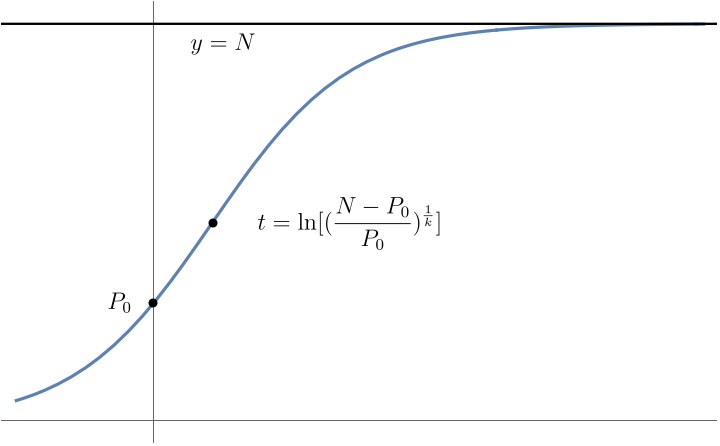
\includegraphics[width=10cm]{misc/logisticmodel.png}
        \caption{$y(t) = \frac{N}{1+be^{-kt}}, b = \frac{N-P_0}{P_0}$}
        \label{fig:logisticmodel}
    \end{figure}
\end{itemize}

% aka "model 4"
\subsection{Linear Equations}

A \textbf{first-order linear differential equation} is a differential equation of the general form:

$$\frac{dy}{dx} + P(x)y = Q(x)$$,

where $P$ and $Q$ are continuous over a particular interval. Notice that this form \textit{does not} fit the form of a separable equation (see \ref{sec:separable}), and thus is not solvable using the same method.

Instead, we have to use a new function, called an \textbf{integrating factor}, called $I(x)$, which will make the equation solvable for $y$. To understand the motivation behind $I(x)$, recall the product rule for calculating derivatives:

$$(xy)' = xy'+y$$

We can define $I(x)$ as a factor such that the left-hand side of the general equation becomes the derivative of $I(x)y$, and simplifies as follows:

\begin{equation}
    \begin{split}
    I(x)(\frac{dy}{dx} + P(x)y) = (I(x)y)' &= I(x)Q(x)\\
    \int (I(x)y)' &= \int I(x)Q(x) dx\\
    I(x)y &=  \int I(x)Q(x) dx + C\\
    y(x) &= \frac{1}{I(x)}[\int I(x)Q(x) dx + C]\\
    \end{split}
\end{equation}

This provides a general solvable form for the equation, but we still need to find $I(x)$ to make this useful. We can do so by rearranging $I(x)(\frac{dy}{dx} + P(x)y) = (I(x)y)'$ as follows:

\begin{equation}
    \begin{split}
    I(x)(\frac{dy}{dx} + P(x)y) = I(x)(y'+P(x)y) &= (I(x)y)'\\
    I(x)y' + I(x)P(x)y &= I'(x)y+I(x)y'\\
    I(x)P(x)y &= I'(x)y\\
    I(x)P(x) &= I'(x)\\
    \end{split}
\end{equation}

This is just a separable equation, which can be solved for $I$:

\begin{equation}
    \begin{split}
        \int \frac{dI}{I} &= \int P(x) dx\\
        \ln |I| &= \int P(x) dx \\
        I  &= \pm e^{\int P(x) dx + C} = Ae^{\int P(x) dx}, A=\pm e^{C}\\
    \end{split}
\end{equation}

We can typically set $A=1$ for a general $I$. Using these general steps, we can thus solve a linear first-order differential equation by multiplying it by the appropriate integrating factor $I(x) = e^{\int P(x) dx}$. For instance, to solve $x^2y'+xy=1$:

\begin{equation}
    \begin{split}
        x^2y'+xy &= 1\\
        y' + \frac{1}{x}y &= \frac{1}{x^2}\\
        I(x) &= e^{\int \frac{1}{x} dx} = e^{\ln x} = x\\
        I(x)(y' + \frac{1}{x}y) &= I(x)\frac{1}{x^2}\\
        xy'+y &= \frac{1}{x}\\
        (xy)' &= \frac{1}{x}\\
        \int (xy)' &= \int \frac{1}{x} dx\\
        xy &= \ln x + C\\
        y &= \frac{\ln x + C}{x}\\
    \end{split}
\end{equation}

Note that the original equation was not in standard form, but we were able to simply divide each factor by $x^2$ to get it into standard form.

\subsection{Orthogonal Families of Curves}

Using differential equations, we can determine the general equation of curves orthogonal (ie "perpendicular") to a given curve (or, typically, a family of curves). Consider the general family of curves described by;

$$ax^2+by^2=k,$$

where $a,b,k$ are real constants. The derivative of any perpendicular curve must be the negative reciprocal of the derivative of the original curve (by the very definition of perpendicularity), so we can find the derivative of the original curve as follows, using implicit differentiation:

\begin{equation}
    \begin{split}
        ax^2+by^2 &= k\\
        2ax + 2by\dydx &= 0\\
        \dydx &= \frac{-2ax}{2by} = -\frac{ax}{by}\\
        \therefore m_{orth.} &= -(\dydx)^{-1} = \frac{by}{ax}\\
    \end{split}
\end{equation}

If we define $P$ as the orthogonal curve's $y$-value, we can then find a general equation for the orthogonal curve as a function of $x$ by rewriting it as a (\textit{separable}) differential equation:

\begin{equation}
    \begin{split}
        \frac{dP}{dx} &= m_{orth.} = \frac{by}{ax} = \frac{bP}{ax}\\
        \frac{dP}{bP} &= \frac{dx}{ax}\\
        \int \frac{dP}{bP} &= \int \frac{dx}{ax}\\
        \frac{1}{b}\ln |P| &= \frac{1}{a}\ln |x| + C\\
        \ln |P| &= \frac{b}{a}\ln|x|+C\\
        P(x) = Ke^{\ln |x^{\frac{b}{a}}|} &= Kx^{\frac{b}{a}}, K = \pm e^{C}\\
    \end{split}
\end{equation}

This general method can be used to find the general equation of any curve orthogonal to a given curve (assuming the given curve is differentiable). See figure \ref{fig:orthogonalcurves} for a visualization of this concept.

\begin{figure}[!ht]
    \centering
    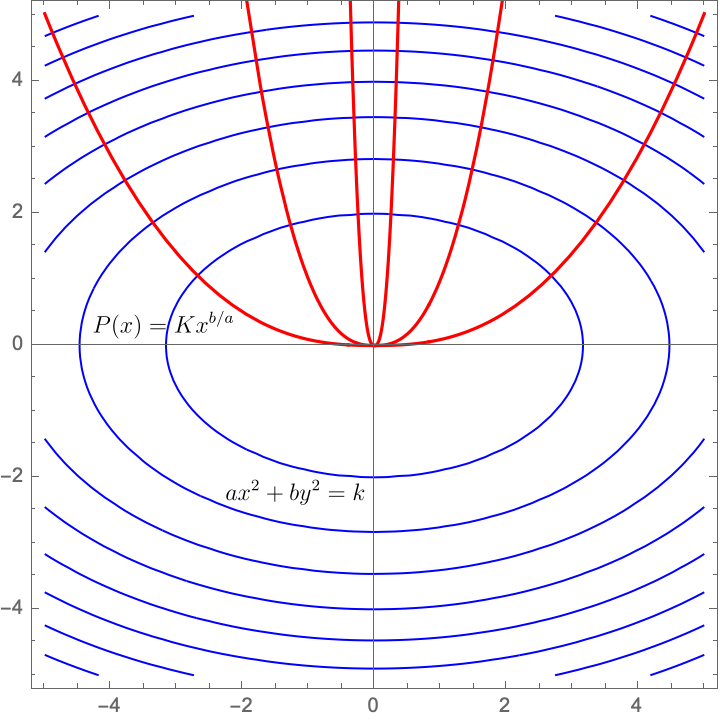
\includegraphics[width=7.8cm]{misc/orthogonalcurves.png}
    \caption{$ax^2+by^2=k$ and its orthogonal curves}
    \label{fig:orthogonalcurves}
\end{figure}

\section{Multivariable Calculus}

\subsection{Introductions/Visualizations}

Numerous real-world concepts can be described as function of multiple variables. A function of two variables, for instance, can be defined as a $f(x,y)$. 

\begin{figure}[!ht]
    \centering
    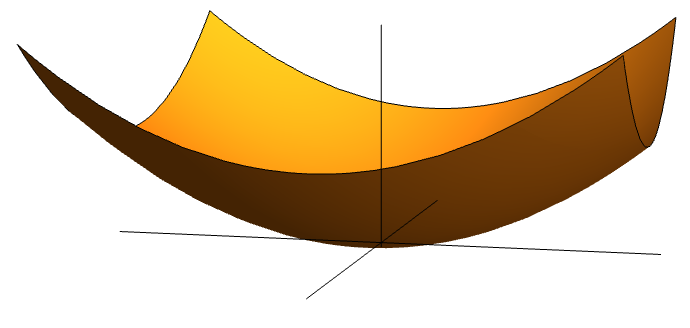
\includegraphics[width=8.5cm]{misc/xsquaredysquared.png}
    \caption{$f(x,y)=x^2+y^2$}
    \label{fig:2dfunction}
\end{figure}

Functions of many variables can often be difficult to visualize (particularly of more than 2 variables), but at least for a function of two variables, we can visualize it as a surface in 3D. For instance, consider the function $f(x,y) = x^2 + y^2$, and figure \ref{fig:2dfunction}.

\begin{figure}
    \centering
    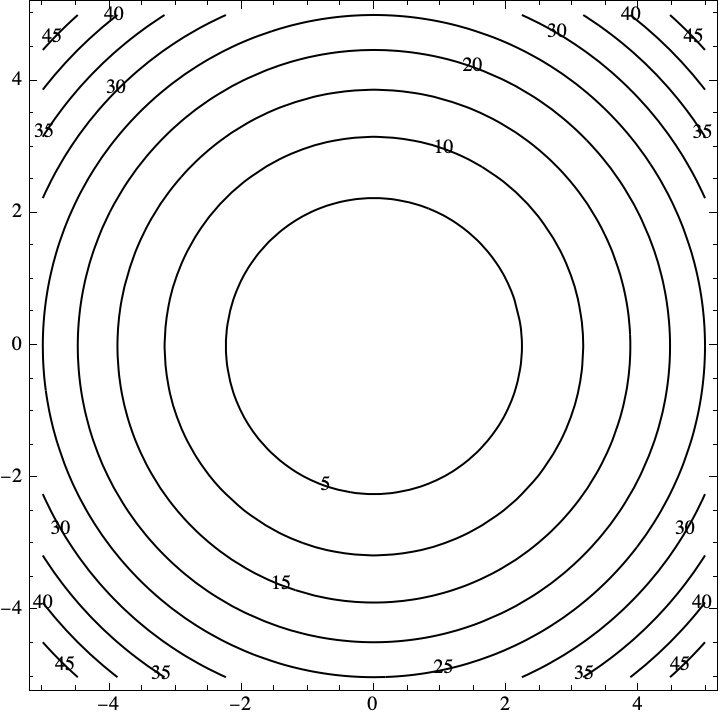
\includegraphics[width=6.5cm]{misc/levelcurves.png}
    \caption{Level curves of $f(x,y) = x^2 + y^2$}
    \label{fig:levelcurves}
\end{figure}

While this is helpful, 3D plots aren't always realistic to use to visualize a function. Instead, we can draw \textbf{level curves}, by plotting a number of curves of a constant $z$-value in the standard $x-y$ plane. See figure \ref{fig:levelcurves} for a level curve graph of $f(x,y) = x^2 + y^2$. Note that, visually, this plot is essentially the same as looking at the surface of the function in 3D from above the $z$-axis.

Note that, while harder to visualize, functions of more than two variables can be described similarly. For instance, a function of three variables can be described as a surface in 4D, and a function of four variables can be described as a surface in 5D, and so on. By extension, we can also describe the level curves of a function of $n$ variables as a family of functions in $n$ (ie a function of 3 variables can be visualized as a level plot in 3D).

\subsection{Limits}

A limit of a function of multiple variables is described as the value of the said function when all of its variables approach a particular coordinate. For the function $f(x,y)$, for example, we can write its limit as it approaches some point $(a,b)$:

$$\lim_{(x,y)\to(a,b)}f(x,y)$$

Determining limits (and in particular, if a limit exists) is not quite as straightforward as for functions of a single variable. For a function $f(x)$ and a point $a$, for instance, if the limit approaching from the right ($a^{+}$) doesn't equal the limit approaching from the left ($a^{-}$), then the limit doesn't exist. For a function of two variables, though, a limit can be approached from an infinite number of directions, assuming the corresponding $(x,y)$ is still in the domain of the function. By extension, we can only say that a limit exists in this case if, no matter which direction we approach the limit from, the limit is the same.

We can use, however, the precise definition of a limit to more accurately define a limit of $f(x,y)$ with domain $D$ as it approaches $(a,b)$:

$$\lim_{(x,y)\to(a,b)} f(x,y) = L$$

if for every $\epsilon > 0$, there exists a $\delta >0$ such that if $(x,y)\in D$ and $0<\sqrt{(x-a)^2+(y-b)^2}<\delta$, then $|f(x,y)-L|<\epsilon$.

By extension of this definition of a limit, we can say a function $f(x,y)$ is continuous at $(a,b)$ if $\lim_{(x,y)\to(a,b)} f(x,y) = f(a,b)$, very similarly to the definition of continuity for a function of a single variable.

\subsection{Partial Derivatives}

Extending the definition of a derivative of a function of 1 variable, we can find the \textbf{partial derivative} of a function of multiple in terms of a particular variable (notated as $\frac{\partial f}{\partial x}$ or $f_x(x,y)$), while treating the other variable(s) as a constant:

\begin{equation}
    \begin{split}
        f_x(x,y) = \frac{\partial f}{\partial x} = \lim_{h\to0}[ \frac{f(x+h,y)-f(x,y)}{h}]\\
        f_y(x,y) = \frac{\partial f}{\partial y} = \lim_{h\to0}[ \frac{f(x,y+h)-f(x,y)}{h}]
    \end{split}
\end{equation}

This definition can, naturally, be extended to higher derivatives. Just as there were two partial derivatives for $f(x,y)$ depending on which variable $f$ was being differentiated in respect to, there are similarly two second partial derivatives for each first partial derivative (and a similar pattern follows for functions of a higher number of variables). For $f(x,y)$, it can be said:

\begin{equation}
    \begin{split}
      (f_x)_x &= f_{xx} = \frac{\partial}{\partial x}(\frac{\partial f}{\partial x}) = \frac{\partial^2f}{\partial x^2}\\
      (f_x)_y &= f_{xy} = \frac{\partial}{\partial y}(\frac{\partial f}{\partial x}) = \frac{\partial^2f}{\partial y \partial x}\\
    (f_y)_x &= f_{yx} = \frac{\partial}{\partial x}(\frac{\partial f}{\partial y}) = \frac{\partial^2f}{\partial x \partial y}\\
    (f_y)_y &= f_{yy} = \frac{\partial}{\partial y}(\frac{\partial f}{\partial y}) = \frac{\partial^2f}{\partial y^2}
    \end{split}
\end{equation}


\begin{shaded*}
    \textbf{Clairaut's Theorem:} 
    
    If the point $(a,b)$ is in the domain of $f(x,y)$, and $f_{xy}$ and $f_{yx}$ are continuous, then $f_{xy}(a,b)=f_{yx}(a,b)$.
\end{shaded*}

\subsection{Differentials, Errors, Approximations}

In functions of a single variable, it can be said:

\[
    dy = f'(x) dx    
\]

Similarly, in a function of multiple variables (say $z = f(x,y)$), we can say:

\begin{equation}
    \begin{split}
    dz &= f_x(x,y) dx + f_y(x,y) dy\\
    &= \pd{z}{x} dx + \pd{z}{y} dy
    \end{split}
\end{equation}

Similarly to how the approximate error $\Delta f$ in a function $f(x)$ can be estimated from the value of $\Delta x$ by calculating $\Delta f \approx df =  f'(x) dx$, we can similarly estimate the error in a function of multiple variables by calculating:

\begin{equation}
    \begin{split}
     dz &= \pd{z}{x} dx + \pd{z}{y} dy\\
    \Delta z &= \pd{z}{x} \Delta x + \pd{z}{y} \Delta y   
    \end{split}
\end{equation}

\subsection{Partial Differential Equations}

Just as a \textit{differential equation} relates a function with its derivative(s), a \textit{partial differential equation} relates a multi-variable function with its partial derivatives. 

One of the most notable of these is the \textbf{Laplace equation},

\begin{equation}
    \begin{split}
        \frac{\partial^2u}{\partial x^2} + \frac{\partial^2u}{\partial y^2} = 0
    \end{split}
\end{equation}

with applications in various fields. 

\subsection{Tangents, Linear Approximations}

Just as it is possible to find the \textit{tangent line} to a particular function $f(x)$ by finding the slope $m=f'(a)$ at some point $a$, we can find the \textit{tangent plane} to a function $f(x,y)$ at a particular point $(a,b,c)$. In general, such a plane can be defined as:

\begin{equation}
    \begin{split}
        z - c &= m_x(x-a) + m_y(y-b)\\
        z - c &= f_x(a,b)(x-a) + f_y(a,b)(y-b)
    \end{split}
\end{equation}

Note the similarities between using this equation and the linear equation $y=mx+b$ when finding the tangent line to a function of a single variable.

We can also use the tangent plane to a function $f(x,y)$ to define a linear approximation (or, more accurately, tangent approximation) $L(x,y)$:

\begin{equation}
    \begin{split}
        L(x,y) &= f(a,b) + f_x(a,b)(x-a) + f_y(a,b)(y-b)\\
    \end{split}
\end{equation}

The derivation of this equation is very similar to that of a single-variable linearization. It should be clear that this is simple the equation for the tangent plane at a particular point $(a,b)$, simply rewritten as a function of $x$ and $y$.

\subsubsection{Normal Equation to a Plane}

Using the general form of a tangent plane ($z = ax + by + c$), we can find the normal equation to the the plane at which it is tangent to the original function fairly easily. Rewriting this equation, we can say:

\begin{equation}
    \begin{split}
        z &= ax + by + c\\
        z &- ax - by = c\\
    \end{split}
\end{equation}

One property of the function in this form is that a vector that is perpendicular to it can be written using the coefficients of each variable, ie $\vec{n} = \langle -a, -b,1 \rangle$ (this can fairly easily be proven). From here, we can find a set of functions in terms of (for instance) $t$ that parametrically describe the general normal equation. The slope in each direction $x, y,z$ must be the same as the respective quantity in our normal vector $\vec{n}$, so we can say:

\begin{equation}
    \begin{split}
        x &= -at\\
        y &= -bt\\
        z &= t
    \end{split}
\end{equation}

This form assumes that the original tangent plane in question is at the origin, but can be easily modified to account for a different point, say at $(x,y,z) = (m,n,p)$:

\begin{equation}
    \begin{split}
        x &=m-at\\
        y &= n-bt\\
        z &= p+t
    \end{split}
\end{equation}


% ! in tangent plane section should add part about how you can find the normal line parametrically using the tangent plane

% ! should probably add a section here about differentials
% ! from there can add error

\subsection{The Chain Rule}

The chain rule for derivatives of functions of 1 variable describes the derivative of a composition of two functions; say $y=f(x)$ and $x=g(t)$ (assuming $f$ and $g$ are differentiable), then the derivative of $y$ with respect to $t$ can be described as:

\begin{equation}
    \begin{split}
       \frac{dy}{dt} &= \frac{dy}{dx}\frac{dx}{dt}\\
        (f(g(t)))' &= f'(g(t))g'(t)
    \end{split}
\end{equation}

This is extendable to functions of multiple variables, though with some caveats. In general, though, if $u$ is a function of $n$ variables $x_1, x_2, \dots, x_n$, and each $x$ is a (differentiable) function of $m$ variables $t_1, t_2, \dots, t_m$, then $u$ is also a function of $t_1, t_2, \dots, t_m$, and the derivative of $u$ with respect to $t_i$ can be described as:

\begin{equation}
    \begin{split}
        \frac{\partial u}{\partial t_i} &= \frac{\partial u}{\partial x_1}\frac{\partial x_1}{\partial t_i} + \frac{\partial u}{\partial x_2}\frac{\partial x_2}{\partial t_i} + \dots + \frac{\partial u}{\partial x_n}\frac{\partial x_n}{\partial t_i}\\
        &= \sum_{j=1}^m \frac{\partial u}{\partial x_j}\frac{\partial x_j}{\partial t_i}
    \end{split}
\end{equation}

This general form can seem quite daunting, but can be simplified down to a couple of main cases:

\subsubsection*{\texorpdfstring{Case 1: $u=z=f(g(t),h(t))$}{TEXT}}

Say $u = z = f(x,y)$, where $x = g(t)$ and $y = h(t)$. We can then write:

\begin{equation}
    \begin{split}
        \frac{dz}{dt} = \frac{\partial f}{\partial x} \frac{dx}{dt} + \frac{\partial f}{\partial y}\frac{dy}{dt}
    \end{split}
\end{equation}

\subsubsection*{\texorpdfstring{Case 2: $u=z=f(g(s,t),h(s,t))$}{TEXT}}

Say $u = z = f(x,y)$, where $x = g(s,t)$ and $y = h(s,t)$. We can then write:

\begin{equation}
    \begin{split}
        \frac{\partial z}{\partial s}&=\frac{\partial z}{\partial x} \frac{\partial x}{\partial s}+\frac{\partial z}{\partial y} \frac{\partial y}{\partial s}\\
        \frac{\partial z}{\partial t}&=\frac{\partial z}{\partial x} \frac{\partial x}{\partial t}+\frac{\partial z}{\partial y} \frac{\partial y}{\partial t}
    \end{split}
\end{equation}

Notice that Case 2 demonstrates the equation for \textit{two} partial derivatives. By extension, the more variables that $u$ is a function of, the more partial derivatives there will be; in this situation, further "cases" simply follow the general aforementioned. 

For example, if $z = e^x \sin y$, $x = st^2$, and $y = s^2t$, then:

\begin{equation}
    \begin{split}
        \pd{z}{s} &= \pd{z}{x} \pd{x}{s} + \pd{z}{y} \pd{y}{s}\\
        &= \pd{}{x}(e^x \sin y) \pd{}{s}(st^2) + \pd{}{y}(e^x \sin y) \pd{}{s}(s^2t)\\
        &= (e^x \sin y)(t^2) + (e^x \cos y)(2st)\\
        &= (e^{st^2} \sin(s^2t))(t^2) + (e^{st^2} \cos(s^2t))(2st)\\
        &= t^2 e^{s t^2} \sin(s^2 t)+2 s t e^{s t^2} \cos(s^2 t)
    \end{split}
\end{equation}

The same method can be used to find $\pd{z}{t}$.

\begin{figure}[!ht]
    \centering
    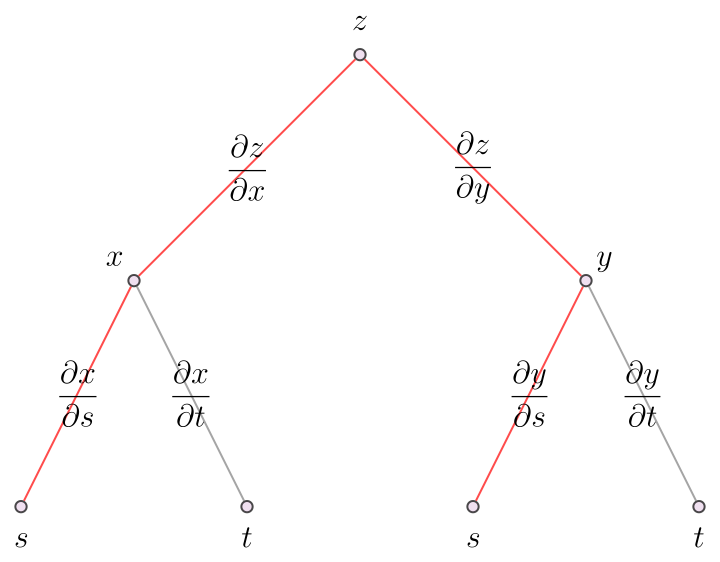
\includegraphics[width=8.0cm]{misc/partialderivativetreegraph.png}
    \caption{Tree graph for the partial derivative of $z = f(x(s,t),y(s,t))$.}
    \label{fig:partialderivativetreegraph}
\end{figure}


\begin{figure}[!ht]
    \centering
    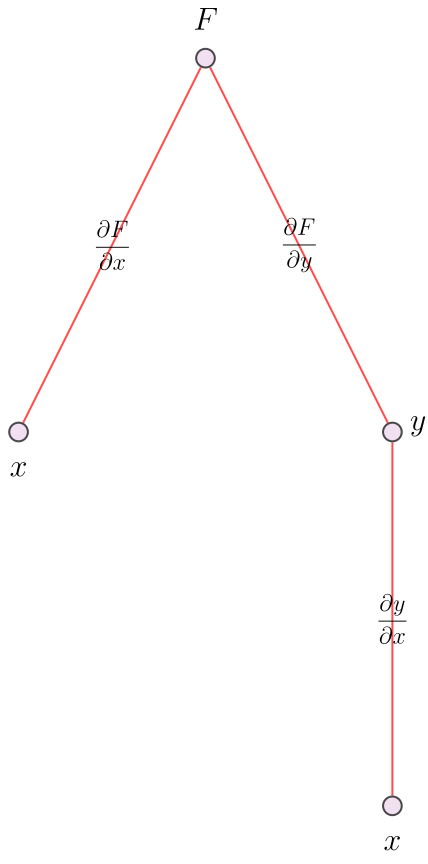
\includegraphics[width=3.0cm]{misc/pdtreeimplicity.png}
    \caption{Tree graph for $F(x,f(x))$.}
    \label{fig:pdtreeimplicit}
\end{figure}

\subsubsection{Tree Graphs}

Using the chain rule for implicit functions of many variables can easily become very confusing. It can help to create a tree graph to visualize the relationships between the functions at hand. For example, for the example above, where $z = f(x(s,t),y(s,t))$, we create a tree graph as in figure \ref{fig:partialderivativetreegraph}.


To find, for instance, $\pd{z}{s}$, you follow the path from $z$ to each $s$ in the tree graph, and multiply the partial derivatives of each function along the way (note the highlighted branches). In this case, $\pd{z}{s} = \pd{z}{x} \pd{x}{s} + \pd{z}{y} \pd{y}{s}$.

% add proof of chain rule for multivariable functions?

% add implicit differentiation here
\subsection{Implicit Differentiation}

Given a function in the form $F(x,y) = 0$ where $y$ is a function $f$ of $x$ (ie $F = (x,f(x))$), we can differentiate both sides in terms of $x$, using the chain rule (see figure \ref{fig:pdtreeimplicit}):


\begin{equation}
    \begin{split}
        F(x,y) &= 0\\       
        \pd{F}{x} \frac{dx}{dx} +\pd{F}{y}\dydx &= 0\\
        \pd{F}{x} + \pd{F}{y}\frac{dy}{dx} &= 0\\
        \dydx = -\frac{\pd{F}{x}}{\pd{F}{y}} &= -\frac{F_x}{F_y}
    \end{split}
\end{equation}

\textit{Note that $\frac{dx}{dx} = 1$, as we can think of $x$ as a function of $x$ (ie $x = x$).} The proof for functions of more variables is fairly similar; for a function of the form $F(x,y,z)=0$ where $z = f(x,y)$, we can find $\pd{z}{x}$:

\begin{equation}
    \begin{split}
        F(x,y,z) &= 0\\
        \pd{F}{x}\pd{x}{x} + \pd{F}{y}\pd{y}{x} + \pd{F}{z}\pd{z}{x} &= 0\\
        \pd{x}{x} = 1, \pd{y}{x} &= 0\\
        \pd{F}{x} + \pd{F}{z}\pd{z}{x} &= 0\\
        \therefore \pd{z}{x} &= -\frac{\pd{F}{x}}{\pd{F}{z}}\\
    \end{split}
\end{equation}

Note that the third line of this proof is valid as $\pd{x}{x} = 1$ as shown above, and $\pd{y}{x} = 0$ because $y$ is not a function of $x$. Finding $\pd{z}{y}$ is incredibly similar (and equals $-\frac{\pd{F}{y}}{\pd{F}{z}}$).

Consider a "simpler" function, $x^2+y^3=0$; differentiating in terms of $x$ gives:

\begin{equation}
    \begin{split}
        F(x,y) = x^2 + y^3 &= 0\\
        \frac{dy}{dx} &= -\frac{\pd{F}{x}}{\pd{F}{y}}\\
        &= -\frac{2x}{3y^2}\\
    \end{split}
\end{equation}
% directional derivatives, gradient, probably go in the same section
\subsection{Directional Derivatives and the Gradient}

The rate of change (derivative) of a function $f(x,y)$ of 2 variables can theoretically be defined in any arbitrary direction, say, in the direction of a unit vector $\vec{u} = \left\langle a,b\right\rangle$. By this logic, then $f_x(x,y)$ is the derivative in the direction of $\hat{i} = \left\langle 1, 0 \right\rangle$, and $f_y(x,y)$ is the derivative in the direction of $\hat{j} = \left\langle 0, 1 \right\rangle$. The derivative in the direction of any arbitrary unit vector $\vec{u}$ is called a \textit{directional derivative}, and is denoted as $D_{\vec{u}}f(x,y)$. Using the limit definition of a derivative, we can write:

\begin{equation}\label{eqn:directionalderivativelimit}
    \begin{split}
        D_{\vec{u}}f(x_0,y_0) &= \lim_{h\to\infty}[\frac{f(x_0+ah,y_0+bh)-f(x_0,y_0)}{h}]
    \end{split}
\end{equation}

\textit{Note that the top line states $f(x_0+ah,y_0+bh)$ because the function is increasing by $a$ in the $x$ direction and $b$ in the $y$ direction.}

To simplify this, let $g(h) = f(x_0+ah,y_0+bh)$, then we can say, using eqn. \ref{eqn:directionalderivativelimit}:

\begin{equation}
    \begin{split}
        g'(0) &= \lim_{h\to\infty}[\frac{g(h)-g(0)}{h}] = \lim_{h\to\infty}[\frac{f(x_0+ah,y_0+bh)-f(x_0,y_0)}{h}] = D_{\vec{u}}f(x_0,y_0)\\
    \end{split}
\end{equation}

Since $g(h) = f(x_0+ah,y_0+bh)$, we can define $x = x_0+ah$ and $y = y_0+bh$ (ie, $x$ and $y$ are both functions of $h$), and using the chain rule, write:

\begin{equation}\label{eqn:directionalderivativesimplification}
    \begin{split}
        g(h) &= f(x_0+ah,y_0+bh) = f(x(h),y(h))\\
        g'(h) &= \pd{f}{x}\frac{dx}{dh} + \pd{f}{y}\frac{dy}{dh}\\
        \frac{dx}{dh} &= \frac{d}{dh} (x_0+ah) = a\\
        \frac{dy}{dh} &= \frac{d}{dh} (y_0+bh) = b\\
        \therefore g'(h) &= \pd{f}{x}(a) + \pd{f}{y}(b)\\
        &= f_x(x,y)a + f_y(x,y)b\\
        g'(\red{0}) &= f_x(x_0,y_0)a + f_y(x_0,y_0)b\\
        &= D_{\vec{u}}f(x_0,y_0)
    \end{split}
\end{equation}

Note that this last line involves combining the result of calculating $g'(h)$ with the original definition of $g'(0)$ from eqn. \ref{eqn:directionalderivativesimplification}. In summary, if $\vec{u} = \left\langle a, b \right\rangle$, then the derivative of $f(x,y)$ in the direction of $\vec{u}$ is:

\begin{equation}
    \begin{split}
        D_{\vec{u}}f(x,y) &= f_x(x,y)a + f_y(x,y)b
    \end{split}
\end{equation}

Note that this can be rewritten as a \textit{dot product}:

\begin{equation}
    \begin{split}
        D_{\vec{u}}f(x,y) &= f_x(x,y)a + f_y(x,y)b\\
        &= \left\langle f_x(x,y), f_y(x,y) \right\rangle \cdot \left\langle a, b \right\rangle\\
        &= \left\langle f_x(x,y), f_y(x,y) \right\rangle \cdot \vec{u}
    \end{split}
\end{equation}

The first vector in this equation is the \textbf{gradient} (denoted $\nabla$) of $f(x,y)$; specifically:

\begin{equation}
    \begin{split}
        \nabla f(x,y) &= \left\langle f_x(x,y), f_y(x,y) \right\rangle\\
        (&= \pd{f}{x}\hat{i} +\pd{f}{y}\hat{j} )
    \end{split}
\end{equation}

Using this notation, we can simplify the form of the directional derivative to 

\begin{equation}\label{eqn:directionalderivativedefinitiondotproduct}
    \begin{split}
        D_{\vec{u}}f(x,y) = \nabla f(x,y) \cdot \vec{u}
    \end{split}
\end{equation}

In higher dimensions, the same general concepts apply; for instance, $D_{\vec{u}}f(x,y,z) = \nabla f(x,y,z) \cdot \vec{u}$, where $\vec{u}$ is a vector in $\real^3$.

\subsubsection{Maximizing the Gradient}

Given a function, $f(x,y)$, a common question is to find what direction it changes the fastest, ie, what direction should $\vec{u}$ be pointing to maximize $D_{\vec{u}}f(x,y)$? This is fairly simple to calculate using eqn. \ref{eqn:directionalderivativedefinitiondotproduct}'s definition of the gradient:

\begin{equation}
    \begin{split}
        D_{\vec{u}} f(x,y) &= \nabla f(x,y) \cdot \vec{u}\\
        &= |\nabla f(x,y)| |\vec{u}| \cos(\theta)\\
        &= |\nabla f(x,y)| \cos(\theta)\\
    \end{split}
\end{equation}

Since $\cos$ is at a max when $\theta = 0$, we can thus maximize $D_{\vec{u}} f(x,y)$ by setting $\vec{u}$ in the same direction as $\nabla f(x,y)$.

\subsection{Using a Jacobian Matrix}

The Jacobian matrix is a matrix of partial derivatives of a function of multiple variables. It has many more applications beyond the scope of this course, but is still interesting/useful enough to include here. To understand the derivation of the Jacobian matrix, first consider the derivation of Cramer's rule.

\subsubsection{Cramer's Rule}

\textbf{Cramer's Rule} is a general method for solving systems of linear equations, specifically, when there are as many unknowns as there are equations. Its easiest to understand by deriving it first from a simple system of 2 equations (and thus, 2 unknowns):

\begin{equation}
    \begin{split}
        ax + by &= \alpha\\
        cx + dy &= \beta
    \end{split}
\end{equation}

We can cancel out the $y$ terms:

\begin{equation}
    \begin{split}
        \red{d}(ax + by &= \alpha)\\
        \red{b}(cx + dy &= \beta)\\
        (adx + bdy &= d\alpha)\\
        -(cbx + bdy &= b\beta)\\
        \hline
        adx - cbx &= d\alpha - b\beta\\
        x(ad - cb) &= d\alpha - b\beta\\
        x &= \frac{d\alpha - b\beta}{ad - cb}
    \end{split}
\end{equation}

If we consider $A$ as the matrix of coefficients of the system and $B$ as the matrix with the first column of $A$ replaced with the column vector $\left\langle \alpha, \beta \right\rangle$ (ie the solutions), then we can write the above as:

\begin{equation}
    \begin{split}
        A = \begin{bmatrix}
            a & b\\
            c & d
        \end{bmatrix}
        \quad&
        B = \begin{bmatrix}
            \alpha & b\\
            \beta & d
        \end{bmatrix}
        \quad\\
        x &= \frac{d\alpha - b\beta}{ad - cb} = \frac{det(B)}{det(A)}
    \end{split}
\end{equation}

Cramer's Rule in general states that for an equation $Ax = b$, $x_i = \frac{det(B_i)}{det(A)}$, where $B_i$ is the matrix with the $i^{th}$ column of $A$ replaced with $b$ and $x_i$ is the $i^{th}$ variable in the equation(s). See \hyperref{http://notes.louismeunier.net/Linear%20Algebra/linearalgebra.pdf}{}{}{here} for more Linear Algebra.

\subsection{Using Cramer's Rule to Derive the Jacobian Matrix}






% ! NOTES/TODO
\iffalse
   Add arc length, but should probably go into the application of integration stuff (which really hasn't been covered yet lol)
   Add jacobian matrix + cramer's rule
\fi
\end{document}